% Preamble ==================================================================
\documentclass[11pt]{article}
\usepackage{geometry}
\geometry{verbose,tmargin=2.5cm,bottom= 1.5cm,lmargin=2.5cm,rmargin=2.5cm}
\usepackage{float}
\usepackage{graphicx}
\usepackage{amsmath}
\usepackage{amssymb}
\usepackage{enumitem}
\usepackage{mathtools}
\usepackage{mathrsfs}

\usepackage{tensor}
\usepackage{cancel}
\usepackage{wasysym}
\usepackage{braket}

\usepackage{amsthm} % theorem

\numberwithin{equation}{section}

\usepackage{titlesec,dsfont}

%Format section heading style
\usepackage{sectsty}
\sectionfont{\sffamily\bfseries\large}
\subsectionfont{\sffamily\normalsize\slshape}
\subsubsectionfont{\sffamily\small\itshape}
\paragraphfont{\sffamily\small\textbf}


%Put period after section number
\makeatletter
\def\@seccntformat#1{\csname the#1\endcsname.\quad}
\makeatother

%Bibliography
\usepackage[round]{natbib}
\bibliographystyle{genetics}

%Format captions
\usepackage[ labelsep=period, justification=raggedright, margin=10pt,font={small},labelfont={small,normal,bf,sf}]{caption}

\setlength{\parskip}{0ex} %No space between paragraphs.

\renewcommand{\familydefault}{\sfdefault}

\newcommand\indep{\protect\mathpalette{\protect\independenT}{\perp}}
\newcommand{\nindep}{\not\!\perp\!\!\!\perp}
\def\independenT#1#2{\mathrel{\rlap{$#1#2$}\mkern2mu{#1#2}}}

%PUT ME LAST--------------------------------------------------
\usepackage[colorlinks=true
,urlcolor=blue
,anchorcolor=blue
,citecolor=blue
,filecolor=blue
,linkcolor=black
,menucolor=blue
,linktocpage=true
,pdfproducer=medialab
,pdfa=true
]{hyperref}

\makeatother %Put this last of all

% Symbol definitions
\newcommand{\defeq}{\coloneqq}
\renewcommand{\d}[1]{\ensuremath{\operatorname{d}\!{#1}}}
\newcommand{\dpow}[2]{\ensuremath{\operatorname{d}^{#2}\!{#1}}}
\newcommand{\deriv}[2]{\frac{\ensuremath{\operatorname{d}\!{#1}}}{\ensuremath{\operatorname{d}\!{#2}}}}
\newcommand{\pderiv}[2]{\frac{\ensuremath{\partial}{#1}}{\ensuremath{\partial}{#2}}}
\newcommand{\derivn}[3]{\frac{\ensuremath{\operatorname{d}^{#1}\!{#2}}}{\ensuremath{\operatorname{d}\!{#3}^{#1}}}}
\DeclareMathOperator{\diag}{diag}
\DeclareMathOperator{\tr}{tr}
\newcommand{\tn}[2]{\tensor{#1}{#2}}

% Make theorems bold
\makeatletter
\def\th@plain{%
  \thm@notefont{}% same as heading font
  \itshape % body font
}
\def\th@definition{%
  \thm@notefont{}% same as heading font
  \normalfont % body font
}
\makeatother

% Theorem definitions
\newtheorem{thm}{Theorem}[section]
\newtheorem{defn}{Definition}[section]
\newtheorem{cor}{Corollary}[section]
\newtheorem{prop}{Property}[section]
\newtheorem{rle}{Rule}[section]
\newtheorem{lma}{Lemma}[section]

\newcommand{\bs}{\boldsymbol}

%Preamble end--------------------------------------------------


\begin{document}



\begin{flushleft}
\textbf{\Large Notes on Physics from Symmetry}
\end{flushleft}

\begin{flushleft}
Author: Juvid Aryaman

Last compiled: \today
\end{flushleft}

\noindent This document contains my personal notes on Jakob Schwichtenberg's Physics from Symmetry \citep{Schwichtenberg15}, with a sprinkling of notes from my undergraduate physics course in quantum field theory (and, to a lesser extent, general relativity).


\section{Special relativity}

\subsection{Definitions and postulates} \label{sec:postualtes-sr}

In special relativity, \textbf{inertial frames of reference} are coordinate systems moving with constant velocity relative to each other. Special relativity has two basic postulates:
\begin{enumerate}
\item \textbf{The principal of relativity}: The laws of physics are the same in all inertial frames of reference.
\item \textbf{The invariance of the speed of light}: The velocity of light has the same value $c$ in all inertial frames of reference.
\end{enumerate}

\begin{thm}[Invariant of special relativity]\label{thm:invariant-sr}
Consider two events $A$ and $B$ in an inertial observer $O$'s frame of reference. Let the time interval measured by $O$ between the two events be $(\Delta t)$, and the three spatial intervals be $(\Delta x)$, $(\Delta y)$, $(\Delta z)$. Then, the quantity
\begin{equation}
(\Delta s)^2 \defeq (\Delta c t)^2 - (\Delta x)^2 - (\Delta y)^2 - (\Delta y)^2
\end{equation}
is \textbf{invariant} between all frames of reference. I.e.
\begin{equation}
(\Delta s') = (\Delta s)
\end{equation}
for any inertial frame of reference $O'$.
\end{thm}
\noindent Theorem \ref{thm:invariant-sr} follows directly from the invariance of the speed of light (consider a pair of mirrors, for two observers with relative velocity).

\begin{defn}[Proper time] \label{defn:proper-time}
Proper time, $\tau$, is the time measured by an observer in the special frame of reference where the object in question is at rest. In this frame of reference,
\begin{equation}
(\Delta s)^2 = (c \Delta \tau)^2.
\end{equation}
In the infinitesimal limit
\begin{equation}
(\d s)^2 = (c \d \tau)^2.
\end{equation}
\end{defn}
Physically, Defn.~\ref{defn:proper-time} means that all observers agree on the time interval between events for an observer who travels with the object in question. However, different observers \textbf{do not} in general agree on the time interval between events generally: $(\Delta t) \neq (\Delta t')$ -- this is called \textbf{time dilation}. 

\subsection{$c$ is an upper speed limit}
All observers agree on the value of $(\d s)^2=(c \d \tau)^2$. Furthermore, we commonly assume that there exists a minimal proper time of $\tau = 0$ for two events if $\Delta s^2 = 0$. We can therefore write that when $\tau = 0$
\begin{equation}
c^2 = \frac{(\d x)^2 + (\d y)^2 + (\d z)^2}{(\d t)^2}
\end{equation}
between two events with an infinitesimal distance. We can equate the right-hand side with a squared velocity, and hence
\begin{equation}
\tau = 0 \implies c^2 = v^2\ 
\end{equation}
so
\begin{equation}
(\d s)^2 \geq 0 \implies c^2 \geq v^2
\end{equation}
for \textbf{any} pair of events (which are causally connected, although how this follows is not immediately clear to me right now). 

\subsection{Einstein notation}
Moving from left to right, the first index denotes a row, the second index denotes a column, and so on for higher-order tensors. Hence
\begin{equation}
(\boldsymbol{A})_{ij} \defeq \tensor{A}{^i_j}
\end{equation}
where the right hand side is Einstein notation, and the left hand side is usual matrix element notation. 

Throughout this document, where it is instructive to do so, we use a bold symbol (e.g. $\bs{A}$) to stress where we are using conventional matrix notation. We denote the value of the $i$th row and $j$th column of the matrix as $(\bs{A})_{ij}$. However, it is cumbersome and unconventional in the physics community to always denote matrices with a bold symbol, so we often drop the bold symbol and simply denote a matrix $\bs{A}$ as simply $A$. We will, however, \textbf{avoid} writing things like $A_{\mu \nu}$ to denote the $(\mu, \nu)$th element of an arbitrary matrix because such notation has a very particular meaning in Einstein notation. If you see something like $\tensor{A}{_\mu _\nu}$ (i.e. a normal typeface with indices) in this document, then you should assume that we mean what we say\footnote{Unless, of course, I've made a mistake! In which case, my dear reader, you could leave a \href{https://github.com/jaryaman/physics-from-symmetry-notes/issues}{git issue} and I'll do my best to make a fix.} -- in this case $\tensor{A}{_\mu_\nu} = \tensor{A}{^\rho_\nu} \tensor{g}{_\rho_\mu}$ which is \textbf{not} the same as $(\bs{A})_{\mu \nu}$ in general (see below for explanation).

In Einstein notation, we can use the mnemonic ``Upper indices go up to down [column vector, contravariant]; lower indices go left to right [row vector, covariant]''. We commonly use the conventions:
\begin{itemize}
\item Greek letters are used for spacetime components, where indices take values 0, 1, 2, or 3.
\item Latin letters are used for spatial components only, where indices take values 1, 2, or 3.
\end{itemize}
The \textbf{Einstein summation convention} states that where an index appears twice in a single term, and not otherwise defined, it implies summation of that term over all values of the index.

\paragraph{Matrix-vector multiplication} The product of a matrix $A_{ij}$ with a column vector $v_j$ is written as 
\begin{equation}
u^i = \tensor{A}{^i_j} v^j.
\end{equation} 

\paragraph{Matrix multiplication} For a product of two matrices 
\begin{equation}
\tensor{C}{^i_k} = \tensor{A}{^i_j} \tensor{A}{^j_k}  \iff  (\boldsymbol{C})_{ik} = (\boldsymbol{AB})_{ik}.
\end{equation}
The upstairs/downstairs-ness of this equation is irrelevant: what matters is the left/right \textbf{ordering} of the indices, as well as which indices are repeated. For example
\begin{equation}
\tensor{A}{^\mu_\delta} \tensor{\eta}{_\delta _\nu} = (\boldsymbol{A \eta})_{\mu\nu}.
\end{equation}

\paragraph{Transpose} The transpose of a matrix is written as
\begin{equation}
(\boldsymbol{B}^T)_{ij} \defeq (\boldsymbol{B})_{ji} =  \tensor{B}{^j_i} \label{eq:transpose-einstein-notation}
\end{equation}
So, for example
\begin{equation}
\tensor{A}{^\delta_\mu} \tensor{\eta}{_\delta _\nu} = \tensor{(\protect{A^T})}{^\mu_\delta} \tensor{\eta}{_\delta _\nu}  = (\boldsymbol{A^T \eta})_{\mu \nu}. \label{eq:complicated-example-matrix-mul-transp}
\end{equation}

\paragraph{Raising/lowering with metric tensor} In order to be able to freely raise/lower indices (without repeatedly writing the metric tensor), we impose an ordering upon indices of tensor fields -- which we represent typographically with spacing between tensor indices. A metric $g_{ij}$ (or $g^{ij}$) has the effect of lowering (or raising) a repeated index. For example,
\begin{equation}
g_{iq} \tensor{T}{^{abcd}_{efgh}^{ijkl}_{mnop}}  = \tensor{T}{^{abcd}_{efghq}^{jkl}_{mnop}}.
\end{equation}

\subsection{Minkowski spacetime}

\begin{defn}[Four-vector (contravariant)]
A position four-\textbf{vector} is defined as
\begin{equation}
x^\mu = \begin{pmatrix}ct\\x\\y\\z\end{pmatrix} \equiv \begin{pmatrix}x^0\\x^1\\x^2\\x^3\end{pmatrix}.
\end{equation}
\end{defn}
\begin{defn}[Minkowski metric]
The Minkowski metric is defined as 
\begin{equation}
\eta_{\mu \nu} = \diag(1,-1,-1,-1). \label{eq:def-minkowski-metric}
\end{equation}
$\eta$ is used to compute distances and lengths in Minkowski space.
\end{defn}
\noindent We define $\eta^{\mu \nu}$ through the relation
\begin{equation}
\eta^{\mu \nu} \eta_{\nu \sigma} = \tensor{\delta}{^\mu_\sigma}.
\end{equation}


\begin{defn}[One-form (covariant vector)]
We define a one-form as 
\begin{equation}
x_\mu = \eta_{\mu \nu}x^\nu.
\end{equation}
\end{defn} 
\noindent Thus,
\begin{equation}
\d s^2 = \eta_{\mu \nu} \d x^\mu \d x^\nu.
\end{equation}
\begin{defn}[Scalar product]
A scalar product between four-vectors $x$ and $y$ is defined as
\begin{equation}
x \cdot y \defeq x^\mu y^\nu \eta_{\mu \nu} = x_\mu y_\nu \eta^{\mu \nu} = x^\mu y_\mu = x_\nu y^\nu
\end{equation}
due to the symmetry of the metric: $\eta_{\mu \nu} = \eta_{\nu \mu}$.
\end{defn}



\subsection{Lorentz transformations}
From the invariant of SR (Theorem~\ref{thm:invariant-sr}), we have
\begin{equation}
\d s'^2 = \d x'_\mu \d x'_\nu \eta^{\mu \nu} = \d x_\mu \d x_\nu \eta^{\mu \nu}
\end{equation}
for all reference frames. We denote $\Lambda$ as a (1,1) tensor field, which transforms a four-vector from one reference frame to another:
\begin{equation}
\d x'^\mu = \Lambda^\mu{}_{\nu} \d x ^\nu
\end{equation}
which leaves the $\d s^2$ invariant, i.e. $\d s'^2 = ds^2$. It follows that 
\begin{equation}
\eta_{\mu \nu} = \tensor{\Lambda}{^\sigma_\mu} \tensor{\Lambda}{^\delta_\nu} \eta_{\sigma \delta}.  \label{eq:lorentz-tfm-characteristic}\\
\end{equation}
We can write this in ordinary matrix notation using Eq.\eqref{eq:transpose-einstein-notation}
\begin{align}
\eta_{\mu \nu} &= \tensor{\Lambda}{^\sigma_\mu}  \eta_{\sigma \delta} \tensor{\Lambda}{^\delta_\nu} \nonumber \\
\eta_{\mu \nu} &= \tensor{(\Lambda^T)}{^\mu_\sigma}  \eta_{\sigma \delta} \tensor{\Lambda}{^\delta_\nu} \nonumber \\
(\bs{\eta})_{\mu \nu} &= (\bs{\Lambda^T \eta \Lambda})_{\mu \nu} \nonumber \\
\bs{\eta} &= \bs{\Lambda}^T \bs{\eta \Lambda}. \nonumber
\end{align}
The physical meaning of Eq.\eqref{eq:lorentz-tfm-characteristic} is that Lorentz transformations leave the scalar product of Minkowski spacetime invariant: i.e. changes between frames of reference that respect the two postualtes of special relativity (Section~\ref{sec:postualtes-sr}). Conservation of the scalar product is analogous to rigid rotation ($O$) in Euclidean space ($a \cdot b = a' \cdot b' = a^T O^T O b \implies O^T I O = I$), which preserves orientation ($\det(\Lambda)=1$).


Note that $\tensor{\Lambda}{^\mu_\nu} \neq \tensor{\Lambda}{_\nu^\mu}$. Beginning with Eq.\eqref{eq:lorentz-tfm-characteristic},
\begin{align*}
\tensor{\Lambda}{^\mu_\rho} \tensor{\Lambda}{^\nu_\sigma} \eta_{\mu \nu} &= \eta_{\rho \sigma}
\end{align*}
we can raise one index, and lower one index, of $\tensor{\Lambda}{^\nu_\sigma}$
\begin{align}
\tensor{\Lambda}{^\mu_\rho} \eta_{\mu \nu} \tensor{\Lambda}{^\nu_\sigma} \eta_{\nu \mu} \eta^{\sigma \lambda}  &= \eta_{\rho \sigma} \eta_{\nu \mu} \eta^{\sigma \lambda} \nonumber \\
\tensor{\Lambda}{^\mu_\rho} \tensor{\Lambda}{_\mu^\lambda} \cancel{\eta_{\mu \nu}} &=  \cancel{\eta_{\mu \nu}} \tensor{\delta}{_\rho^\lambda} \nonumber \\
\tensor{\Lambda}{^\mu_\rho} \tensor{\Lambda}{_\mu^\lambda} &= \tensor{\delta}{_\rho^\lambda}
\end{align}
so we see that $\tensor{\Lambda}{_\nu^\mu}$ is the inverse of $\tensor{\Lambda}{^\mu_\nu}$.


\section{Lie group theory}
\subsection{Invariance, symmetry, and covariance}
We call a quantity \textbf{invariant} if it does not change under particular transformations. E.g. if we transform $A,B,C,... \rightarrow A',B',C',...$ and we have
\begin{equation}
F(A',B',C',...) = F(A,B,C,...)
\end{equation}
then we say $F$ is invariant under this transformation. \textbf{Symmetry} is defined as invariance under a transformation (or class of transformations). An equation is covariant if it takes the same form when objects in it are transformed. \textit{All physical laws must be covariant under Lorentz transformations.} 

Group theory describes the properties of particular sets of transformations: the invariances under such groups allows us to mathematically describe symmetry. For example, the set of rotations about the origin of a square by $n\pi/2$ form a \textbf{discrete group}, and leave the set of points which constitute the square invariant under the transformation. The set of rotations about the origin of a circle form a \textbf{continuous group}. We can use group theory to work with \textit{all} kinds of symmetries: symmetries which operate on vectors, equations, ...

\subsection{Groups}
\begin{defn}[Group axioms]
A group $(G, \circ)$ is a set $G$, together with a binary operation $\circ$ defined on $G$, that satisfies the following axioms
\begin{itemize}
\item Closure: For all $g_1, g_2 \in G$, $g_1 \circ g_2 \in G$
\item Identity element: There exists an identity element $e \in G$ such that for all $g \in G$, $g \circ e = g = e \circ g$
\item Inverse element: For each $g \in G$, there exists an inverse element $g^{-1} \in G$ such that $g \circ g^{-1} = e = g^{-1}g$.
\item Associativity: For all $g_1, g_2, g_3 \in G$, $g_1 \circ (g_2 \circ g_3) = (g_1 \circ g_2) \circ g_3$
\end{itemize}
\end{defn}

The set of all transformations that leave a given object invariant is called a \textbf{symmetry group}. For Minkowski spacetime, the object that is left invariant is the Minkowski metric, and the corresponding symmetry group is called the \textbf{Poincar\'{e} group}. Notice that the transformations which constitute a group are defined entirely independently from the object on which the transformations act.

\subsubsection{Rotations in two dimensions and $SO(2)$}
Consider the 2D rotation matrix 
\begin{equation}
R_\theta = \begin{pmatrix}
\cos(\theta)& -\sin(\theta)\\
\sin(\theta)& \cos(\theta)
\end{pmatrix} \label{eq:2d-rotation-matrix}
\end{equation}
and the two reflection matrices
\begin{equation}
P_x = \begin{pmatrix}
-1& 0\\
0& 1
\end{pmatrix} \qquad 
P_y = \begin{pmatrix}
1& 0\\
0& -1
\end{pmatrix}.
\end{equation}
These matrices satisfy the group axioms. We can uncover this group from a symmetry perspective. The above transformations leave the length of a vector unchanged, i.e.
\begin{equation}
a.a = a'.a'.
\end{equation}
Letting the transformation be represented by $a' = Oa$, it follows that all members of the group must satisfy
\begin{equation}
O^T O = I.
\end{equation}
This condition defines the group $O(2)$, which is the group of all \textbf{orthogonal} 2$\times$2 matrices. It follows that $\det(O)=\pm 1$ -- i.e. the transformations are area-preserving. The subgroup with $\det(O)=1$ is called $SO(2)$, which corresponds to rigid rotations preserving the orientation of the system -- ``S'' denoting \textbf{special}. 

\subsubsection{Rotations with unit complex numbers and $U(1)$}
A unit complex number is a complex number $z$ which satisfies $|z|^2=z^*z=1$. The group $U(1)$ is the set of unit complex numbers, together with ordinary complex number multiplication. The $U$ stands for `\textbf{unitary}`, which generally stands for the condition 
\begin{equation}
U^\dagger U=1,
\end{equation} 
where $U^\dagger = (U^{T})^*$ is the \textbf{Hermitian conjugate} of $U$. For scalars, the Hermitian conjugate is equivalent to the complex conjugate. Note that a unit complex number can also be denoted as 
\begin{equation}
R_\theta = e^{i\theta} = \cos(\theta) + i \sin(\theta)
\end{equation}
which makes the interpretation of $U(1)$ as rotations on the unit complex numbers evident.

We can connect this description of rotations ($U(1)$) to the previous ($SO(2)$) by defining 
\begin{equation}
1 = \begin{pmatrix}
1 & 0\\
0 & 1
\end{pmatrix}\qquad,\qquad
i = \begin{pmatrix}
0 & -1\\
1 & 0
\end{pmatrix}. \label{eq:map-complex-rot-to-2d-vectors}
\end{equation}
For an arbitrary unit complex number $z = a + ib$, let
\begin{equation}
f(z) = a \begin{pmatrix}
1 & 0\\
0 & 1
\end{pmatrix} + b \begin{pmatrix}
0 & -1\\
1 & 0
\end{pmatrix} = \begin{pmatrix}
a & -b\\
b & a
\end{pmatrix}. \label{eq:isomorphism-so2-u1}
\end{equation}
Since $z = R_\theta = \cos(\theta) + i \sin(\theta)$, we can plug in the real and imaginary components of $z$ into Eq.\eqref{eq:isomorphism-so2-u1} to arrive at Eq.\eqref{eq:2d-rotation-matrix}. We then have $z' = R_\theta z$, to perform rotations. There therefore exists an \textbf{isomorphism} between $SO(2)$ and $U(1)$:
\begin{defn}[Group isomorphism]
Given two groups $(G, *)$, $(H, \astrosun)$, a group isomorphism is a bijective function $f: G \rightarrow H$ such that
\begin{equation}
f(u * v) = f(u) \astrosun f(v) \ \forall\ u, v \in G.
\end{equation}
which is written as
\begin{equation}
(G, *) \cong (H, \astrosun).
\end{equation}
\end{defn}
\noindent $f(z)$ in Eq.\eqref{eq:isomorphism-so2-u1} is therefore a group isomorphism between $U(1)$ and $SO(2)$,
\begin{equation}
SO(2) \cong U(1). \label{eq:so2-is-isomorphic-u1}
\end{equation}
This realization has an analogue in three dimensions, which will reveal something fundamental about nature.

\subsubsection{Rotations in three dimensions and $SO(3)$}
As with $SO(2)$, the defining conditions of $SO(3)$ are
\begin{align}
R^TR &= I \label{eq:def-so3-norm-preserving} \\
\det(R) &= 1. \label{eq:def-so3-parity-preserving}
\end{align}
Matrices satisfying these two conditions represent rigid rotations of 3-dimensional vectors. These matrices can be described by the following three ``basis rotations''
\begin{align}
R_x &= \begin{pmatrix}
1 & 0 & 0 \\
0 & \cos(\theta) & -\sin(\theta) \\
0 & \sin(\theta) & \cos(\theta) \\
\end{pmatrix} \qquad 
R_y = \begin{pmatrix}
\cos(\theta) & 0 & \sin(\theta) \\
0 & 1 & 0 \\
-\sin(\theta) & 0 & \cos(\theta) \\
\end{pmatrix} \nonumber \\
R_z &= \begin{pmatrix}
\cos(\theta) & -\sin(\theta) & 0 \\
\sin(\theta) & \cos(\theta) & 0 \\
0 & 0 & 1
\end{pmatrix}. \label{eq:rotation-matrices-3d}
\end{align}
So, to rotate a vector $v$ around the $z$-axis by $\theta$, we would compute $R_z(\theta) v$. The set of (orientation-preserving) rotation matrices acting on 3-dimensional vectors is called $SO(3)$.

\subsubsection{Quaternions and $SU(2)$}
To get a second description of rotations in three dimensions, we must generalize complex numbers in higher dimensions. Astonishingly, it turns out that there are no 3-dimensional complex numbers. Instead, we can find 4-dimensional complex numbers called quaternions, which will turn out to be able to describe rotations in 3-dimensions. The fact that quaternions are 4-dimensional will reveal something deep about the universe. We could have anticipated this result, because we will be using unit quaternions, which have 3 degrees of freedom.

To construct quaternions, we introduce three complex units satisfying the relations
\begin{align}
\mathbf{i}^2 = \mathbf{j}^2 = \mathbf{k}^2 - -1 \\
\mathbf{ijk} = -1 \\
q = a \mathbf{1} + b\mathbf{i} + c \mathbf{j} + d \mathbf{k}. \label{eq:quaternion-ijk}
\end{align}
All other relations can be computed from the above. For example, the relation $\mathbf{ij}=\mathbf{k}$ can be derived by multiplying both sides of Eq.\eqref{eq:quaternion-ijk} by $\mathbf{k}$. Notice that it follows that the \textbf{basic quaternions} \textbf{anticommute} with each other, see Fig.~\ref{fig:quaternion-multiplication}.

\begin{figure}
\begin{center}
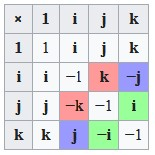
\includegraphics[width=0.2\columnwidth]{figures/quaternion-multiplication.jpg}  
\end{center}
\caption{Quaternion multiplication table, read as row $\times$ column = value. E.g. $\mathbf{ji}=-\mathbf{k}$. In general, the basic quaternions anti-commute.}
\label{fig:quaternion-multiplication}
\end{figure}


The set of unit quaternions satisfy
\begin{align}
q^\dagger q = 1 \\
\implies a^2 + b^2 + c^2 + d^2 = 1.
\end{align}
As the unit complex numbers formed a group under complex number multiplication, the unit quaternions form a group under quaternion multiplication. There are several possible ways of representing the basic quaternions with 2D matrices, but one way is as follows:
\begin{align}
\mathbf{1}&=\begin{pmatrix}
1&0\\
0&1
\end{pmatrix}\qquad,\qquad
\mathbf{i}=\begin{pmatrix}
0&1\\
-1&0
\end{pmatrix} \nonumber \\
\mathbf{j}&=\begin{pmatrix}
0&i\\
i&0
\end{pmatrix}\qquad,\qquad
\mathbf{k}=\begin{pmatrix}
i&0\\
0&-i
\end{pmatrix}. \label{eq:matrix-repn-quaternion}
\end{align}
With these matrices, a generic quaternion $q=a\mathbf{1}+b\mathbf{i}+c\mathbf{j}+d\mathbf{k}$ can be written in a matrix representation as
\begin{equation}
f(q) = \begin{pmatrix}
a+di & b + ci\\
-b + ci & a-di
\end{pmatrix}. \label{eq:quaternion-matrix-repn}
\end{equation}
We also observe that $\det(f(q))=1$, and so we conclude that the unit quaternions are given by the set of matrices with the above form and unit determinant. The unit quaternions, written as 2$\times$2 matrices $U$ therefore fulfil the conditions
\begin{equation}
U^\dagger U=1 \qquad \text{and}\ \det(U)=1. \label{eq:defn-su2}
\end{equation}
\textbf{This defines the symmetry group} $SU(2)$. 

The map between $SU(2)$ and $SO(3)$ is not as simple as the one we saw between $U(1)$ and $SO(2)$. The mapping of a complex number onto a 2-dimensional vector is easy because a complex number has two degrees of freedom: $v=x+\mathbf{i}y$. But the mapping of a quaternion onto 3-dimensional vector is not so straightforward because a quaternion has four degrees of freedom. We will make the mapping of a 3-dimensional vector $(x,y,z)^T$ onto a quaternion $v$ as
\begin{equation}
v \equiv x \mathbf{i} + y \mathbf{j} + z \mathbf{k}.
\end{equation}
Using Eq.\eqref{eq:matrix-repn-quaternion}, we see that $\det(v)=x^2+y^2+z^2$. In order to perform transformations which preserve the length of the vector $(x,y,z)$, we must use transformations which preserve determinants. Therefore, the restriction to \textit{unit} quaternions means that we must restrict to matrices with \textit{unit} determinants\footnote{Since $\det(BA)=\det(B)\det(A)$}. Naively, a first guess would be that simply multiplying a vector $v$ by a unit quaternion $u$ induces a rotation on $v$, but this is not the case because the product of $u$ and $v$ may not belong to $\mathbb{R}\mathbf{i}+\mathbb{R}\mathbf{j}+\mathbb{R}\mathbf{k}$. It turns out that the following transformation can describe rotations in 3-dimensions
\begin{equation}
v'=qvq^{-1}. \label{eq:su2-binary-multiplication}
\end{equation}

Let $t$ be a quaternion defining a rotation through $\phi$, where
\begin{align}
t &= \cos(\frac{\phi}{2}) + \sin(\frac{\phi}{2})u \label{eq:quaternion-3d-rot} \\
u &= u_x \mathbf{i} + u_y \mathbf{j} + u_z \mathbf{k} \\
u^\dagger u &= 1 \implies t^\dagger t = 1.
\end{align}
As an example, suppose we wish to rotate the vector $\vec{v}=(1,0,0)^T$ around the $z$-axis by $\phi$. Then using Eq.\eqref{eq:matrix-repn-quaternion}
\begin{equation}
\vec{v}=(1,0,0)^T \rightarrow v = 1\mathbf{i} + 0 \mathbf{j} + 0 \mathbf{k} = \begin{pmatrix}
0 & 1\\
-1 & 0
\end{pmatrix}.
\end{equation}
From Eq.\eqref{eq:quaternion-3d-rot}, defining $\theta = \phi/2$
\begin{equation}
R_z(\theta)=\cos(\theta) \mathbf{1} + \sin(\theta)\mathbf{k} = \begin{pmatrix}
\cos(\theta) + i \sin(\theta) & 0 \\
0 & \cos(\theta) - i \sin(\theta)
\end{pmatrix}.
\end{equation}
From Eq.\eqref{eq:su2-binary-multiplication}, the rotated vector $v'$ is
\begin{equation}
v' = R_z(\theta) v R_z(\theta)^{-1} = \begin{pmatrix}
0 & \cos(\phi) + i \sin(\phi) \\
-\cos(\phi) + i \sin(\phi) & 0
\end{pmatrix}.
\end{equation}
Using the general quaternion matrix representation Eq.\eqref{eq:quaternion-matrix-repn}, we can equate
\begin{equation}
v'_x = \cos(\phi), \qquad v'_y = \sin(\phi), \qquad v'_z = 0
\end{equation}
as expected.

Inspection of Eq.\eqref{eq:quaternion-3d-rot} reveals that the mapping of unit quaternions onto 3-dimensional rotations is not one-to-one. For example, a rotation by $\phi=\pi$ is equivalent to a rotation by $\phi = 2\pi + \pi = 3\pi$. But,
\begin{align}
t_{\phi=\pi} = \sin(\frac{\pi}{2}) u = u \\
t_{\phi=3\pi} = \sin(\frac{3\pi}{2}) u = -u.
\end{align}
Hence, we call $SU(2)$ a \textbf{double-cover} of $SO(3)$, because every element of $SO(3)$ has two corresponding elements in $SU(2)$ [\textbf{TODO: I think}?]. It is therefore always possible to go unambiguously from $SU(2)$ to $SO(3)$, but not vice versa. 

We will see later that groups which cover other groups are fundamental for quantum spin. Note that the above had one quaternion parameter too many, which may be interpreted as a hint towards relativity: a more natural identification may have been $v=t\mathbf{1}+x\mathbf{i}+y\mathbf{j}+z\mathbf{k}$. Rotations in 4-dimensions require 6 degrees of freedom\footnote{Using ordinary 4$\times$4 matrices, with the constraints $O^TO=1$ and $\det(O)=1$ reduce the 16 components of an arbitrary 4$\times$4 matrix to 6 independent components}. However, there is no 7-dimensional generalisation of complex numbers. But two unit quaternions do have 6 degrees of freedom: we will see later how there is a close connection between two copies of $SU(2)$ and rotations in four dimensions.

\section{Lie algebras}
\subsection{Intuition behind generators}
Consider an element of a continuous group which is arbitrarily close to the identity
\begin{equation}
g(\epsilon) = I + \epsilon X
\end{equation}
where $\epsilon$ is small, and $I$ is the identity (think about 1D rotations for concreteness). We let $X$ remain abstract for the moment. We wish to apply this transformation $N$ times to achieve a finite transformation by a total amount $\theta$, $h(\theta)$. As a result, we may write:
\begin{equation}
h(\theta) = (I + \frac{\theta}{N} X)^N.
\end{equation}
We then take the limit of $N \rightarrow \infty$, which is just the exponential function
\begin{equation}
h(\theta) = \lim_{N \rightarrow \infty} (I + \frac{\theta}{N})^N = e^{\theta X}.
\end{equation}
In this sense, the object $X$ generates the finite transformation $h$, which is why we call $X$ a \textbf{generator}.

We can then differentiate $h(\theta)$ to obtain the generator:
\begin{equation}
X=\left.\deriv{h(\theta)}{\theta}\right|_{\theta=0}. \label{eq:explicit-generator-from-finite-transform}
\end{equation}
If we consider a continuous group of transformations that are given by matrices, we can also make a Taylor expansion of an element of the group about the identity 
\begin{equation}
h(\theta) = \sum_n\frac{1}{n!}\left.\derivn{n}{h}{\theta}\right|_{\theta=0}\theta^n
\end{equation}
which shows how generators generate transformations.

\subsection{An intuitive definition for matrix Lie groups}
For matrix Lie groups, the corresponding Lie algebra can be defined as the collection of objects that give an element of the group when exponentiated. 
\begin{defn}[Lie algebra for matrix Lie groups, non-rigorous]
For a matrix Lie group $G$ (given by $n \times n$ matrices), the Lie algebra $\mathfrak{g}$ of $G$ is given by those $n \times n$ matrices $X$ such that
\begin{equation}
e^{tX}\in G \label{eq:def-generator-lie-matrix-group}
\end{equation}
for $t \in \mathbb{R}$, together with an operation called the Lie bracket, that defines how to combine elements of the Lie algebra
\begin{equation}
[\cdot, \cdot]: \mathfrak{g} \times \mathfrak{g} \rightarrow \mathfrak{g}.
\end{equation}
A Lie algebra is \textbf{closed} under the Lie bracket. 
\end{defn}
Note that, in general $X \circ Y \notin \mathfrak{g}$. 
\begin{thm}
Consider a matrix Lie group $G$ and corresponding Lie algebra $\mathfrak{g}$. If $X, Y \in \mathfrak{g}$ and $g, h \in G$, then
\begin{equation}
g \circ h = e^X \circ e^Y = \underbrace{e^{X + Y + \frac{1}{2}[X,Y]+\frac{1}{12}[X,[X,Y]]-\frac{1}{12}[Y,[X,Y]]+...}}_{\in G} \label{eq:BCH-group-elements-Lie-elements}
\end{equation}
where the right hand side is the Baker-Campbell-Hausdorff formula\footnote{This holds more generally, not only for matrix Lie groups. See also Defn. \ref{defn:Lie-algebra}}. For \textbf{matrix Lie groups}, the Lie bracket $[X,Y]$ is \textbf{equivalent} to the \textbf{commutator} of $X$ and $Y$:
\begin{equation}
[X,Y] = XY - YX.
\end{equation}
Eq.\eqref{eq:BCH-group-elements-Lie-elements} connects combinations of elements of the group $G$ to combinations of elements of the Lie algebra $\mathfrak{g}$.
\end{thm}

\subsection{Generators and Lie algebra of $SO(3)$}
Using the norm-preserving condition of $SO(3)$, Eq.~\eqref{eq:def-so3-norm-preserving}, along with Eq.\eqref{eq:def-generator-lie-matrix-group} $O = e^{\theta J}$, yields
\begin{equation}
O^TO = e^{\theta J^T} e^{\theta J} = 1 \implies J^T + J = 0,
\end{equation}
The parity-preserving condition in Eq.\eqref{eq:def-so3-parity-preserving} also yields\footnote{Because $\det(e^A)=e^{\tr(A)}$}
\begin{equation}
\det(e^{\theta J}) = e^{\theta \tr(J)} = 1 \implies \tr(J) = 0.
\end{equation}
A set of three \textbf{basis}\footnote{i.e. all other generators are linear combinations of the basis generators} generators $J_1, J_2, J_3$ fulfilling both of these conditions can be written conveniently as
\begin{equation}
(J_i)_{jk} = - \epsilon_{ijk},
\end{equation}
where $\epsilon_{ijk}$ is the Levi-Civita symbol
\begin{equation}
\epsilon_{ijk} = \begin{cases} 
1\qquad  &\text{if } (i,j,k)=\{(1,2,3), (2,3,1), (3,1,2)\}\\
0\qquad  &\text{if } i=j\text{ or } j=k\text{ or } k=i\\
-1\qquad &\text{if } (i,j,k)=\{(1,3,2), (2,1,3), (3,2,1)\}\\
\end{cases}.
\end{equation}
The corresponding Lie bracket is 
\begin{equation}
[J_i, J_j] = \epsilon_{ijk} J_k.
\end{equation}
In physics, it is conventional to define the generators of $SO(3)$ with an extra $i$, so that we get Hermitian generators\footnote{i.e. $J^\dagger = J$}, to arrive at
\begin{align}
O &= e^{i \phi J} \label{eq:def-generator-lie-matrix-group-physics} \\
\implies (J_i)_{jk} &= -i \epsilon_{ijk} \\
[J_i, J_j] &= i \epsilon_{ijk} J_k. \label{eq:lie-bracket-so3}
\end{align}
We call the Lie bracket relation of the basis generators \textbf{the} Lie algebra of a given group, because everything that is important about a Lie algebra is encoded in the Lie bracket relation of the basis generators.

An alternative way to derive the basis generators is to begin with the finite transformation matrices and apply Eq.\eqref{eq:explicit-generator-from-finite-transform}. However, the above method is more general, whose steps were: 
\begin{enumerate}[noitemsep]
\item Begin with the definition of the group;
\item Use those constraints to derive the basis generators; 
\item Then derive the an explicit form for finite transformations.
\end{enumerate}

\subsection{Formal definition of a Lie algebra}

\begin{defn}[Lie algebra]
A Lie algebra is a vector space $\mathfrak{g}$ over some field\footnote{Informally, a field is a set, with operations of addition and multiplication defined on that set, along with inverses of those operations} $F$ together with a binary operation $[\cdot, \cdot]: \mathfrak{g} \times \mathfrak{g} \rightarrow \mathfrak{g}$ called the Lie bracket satisfying the following axioms: \label{defn:Lie-algebra}
\begin{enumerate}
\item Bilinearity:
\begin{align}
[aX + bY, Z] &= a[X,Z] + b[Y,Z] \\
[Z, aX + bY] &= a[Z,X] + b[Z,Y]
\end{align}
for all scalars $a,b \in F$ and all elements $X,Y,Z \in \mathfrak{g}$.
\item Anticommutativity:
\begin{align}
[X,Y] = -[Y,X] 
\end{align}
for all $X \in \mathfrak{g}$.
\item The Jacobi identity
\begin{equation}
[X,[Y,Z]] + [Z,[X,Y]] + [Y,[Z,X]] = 0
\end{equation}
for all elements $X,Y \in \mathfrak{g}$.
\end{enumerate}
\end{defn}
Importantly, this definition makes no reference to any Lie group: the definition of a Lie algebra stands on its own.

\subsection{Generators and Lie algebra of $SU(2)$}
Using Equations \eqref{eq:defn-su2} for the definition of $SU(2)$, and Eq.\eqref{eq:def-generator-lie-matrix-group-physics} for the definition of a generator, we arrive at
\begin{equation}
e^{-iJ^\dagger} e^{iJ_i} = e^{-iJ_i^\dagger + iJ_i + \frac{1}{2}[J_i^\dagger, J_i]+...}=1
\end{equation}
where the right-hand side uses the Baker-Campbell-Hausdorff theorem. This implies that
\begin{align}
J = J^\dagger \\
\tr(J)=0
\end{align}
where the second equation uses $\det(U)=1$. A basis for Hermitian traceless 2$\times$2 matrices is given by the 3 \textbf{Pauli} matrices
\begin{equation}
\sigma_1 = \begin{pmatrix}
0&1\\
1&0
\end{pmatrix}, \qquad
\sigma_2 = \begin{pmatrix}
0&-i\\
i&0
\end{pmatrix}, \qquad
\sigma_3 = \begin{pmatrix}
1&0\\
0&-1
\end{pmatrix}.
\end{equation}
We conventionally define 
\begin{equation}
J_i \equiv \sigma_i/2 \label{eq:generator-su2-lie-algebra-2d}
\end{equation}
to arrive at the Lie bracket (or, equivalently, commutator relationship)
\begin{equation}
[J_i, J_k] = i \epsilon_{ijk} J_k \label{eq:lie-bracket-su2}
\end{equation}
which is \textbf{identical} to Eq.\eqref{eq:lie-bracket-so3} for $SO(3)$! Hence we say that $SU(2)$ and $SO(3)$ have the same Lie algebra, since they share the same Lie bracket. 

\subsection{Lie groups and covering groups}
An $SU(2)$ transformation doesn't necessarily have to be represented by 2$\times$2 matrices. An abstract definition of a Lie group will enable us to see the connection between different descriptions of the same transformation. 

A \textbf{Lie group} is a group that is also a differentiable manifold. A Lie group must have the group operations $\circ$ \textbf{induce} a \textbf{differentiable} map of the manifold onto itself. Concretely, this means that every group element, e.g. $A$, induces a differentiable map that takes any element of the group $B$ to another element of the group $C=AB$. 

\begin{defn}[Simply connected Lie group]
A Lie group is said to be simply connected if every closed curve on the manifold can be shrunk smoothly to a point. 
\end{defn}

\begin{thm}[Existence of a covering group]
There exists a unique simply connected Lie group corresponding to each Lie algebra. We call this Lie group the \textbf{covering} group. All other groups having the same Lie algebra are said to be ``covered'' by the simply connected Lie group.\footnote{This is a result from differential geometry.} 
\end{thm}

\begin{defn}[Unit $n$-sphere]
A unit $n$-sphere is denoted as the set of points satisfying
\begin{equation}
S^n=\{x \in \mathbb{R}^{n+1}: ||x||=1\}.
\end{equation}
\end{defn}

$S^n$ is therefore a sphere embedded in $n+1$ dimensions, but with a unit radius constraint, implying an $n$-dimensional object. For groups we have discussed so far, we may identify:
\begin{enumerate}
\item $S^1$, with group operation of multiplication, is the covering group of 1-dimensional rotations. $S^1 \cong U(1) \cong SO(2)$.
\item $S^3$, with group operation of multiplication, is the covering group of 3-dimensional rotations. $S^3 \cong SU(2) \underbrace{\rightarrow}_{\text{two-to-one}}SO(3)$.
\end{enumerate}
Geometrically, we can think of $SO(3)$ as a 3-sphere but with antipodal points identified: this is because each point of $SO(3)$ is associated with two points of $SU(2)$ which is equivalent to $S^3$. 

\subsection{Representation theory}

Representation theory deals with \textit{representing} abstract algebraic structures (mainly groups, associative algebras, and Lie algebras) with linear transformations of vector spaces -- i.e. matrices operating on columnar vectors. Considering just groups for now, a representation abides the following definition
\begin{defn}[Representation for a group]
A representation is a map $R$ (or \textbf{homomorphism}) between any group element $g$ of a group $G$ onto a vector space $V$ such that:
\begin{itemize}[noitemsep]
\item $R(e) = I$, i.e. the identity element of the group is also the matrix identity
\item $R(g^{-1})=(R(g))^-1$, i.e. inverse elements are mapped to inverse transforms
\item $R(g) \circ R(h) = R(gh)$.
\end{itemize}
\end{defn}

For example, the usual rotation matrices in Eq.\eqref{eq:rotation-matrices-3d} are a representation of the group $SO(3)$ on the vector space $\textbf{R}^3$. Representation theory allows us to examine the effect of the group on other vector spaces -- of potentially different dimensionality than the definition of the group itself.

\begin{thm}[Similarity transformation]
If $R$ is a representation of group $G$ with elements $g$, then for any invertible matrix $S$,
\begin{equation}
R'(g) = S^{-1}R(g)S
\end{equation}
is also a representation.
\end{thm}
\begin{proof}
Follows immediately from the definition of a representation. For example,
\begin{equation}
R'(g_1)R'(g_2) = S^{-1}R(g_1)SS^{-1}R(g_2)S = S^{-1}R(g_1)R(g_2)S = S^{-1}R(g_1 g_2)S = R'(g_1 g_2).
\end{equation}
\end{proof}
This freedom to perform similarity transformations corresponds to the freedom to choose a basis for the vector space the group acts on.

\begin{defn}[Invariant subspace]
Given a representation $R$ of a group $G$ on vector space $V$, we call $V' \subseteq V$ an invariant subspace if for all $v \in V'$, we have $R(g) \in V'$.
\end{defn}

\begin{defn}[Subrepresentation]
A subrepresentation of a representation $(R, V)$ of a group $G$ is a representation $(R', V')$ such that $V' \subseteq V$ and 
\begin{equation}
R'(g)v = R(g)v
\end{equation}
for all $v \in V'$.
\end{defn}

\begin{defn}[Irreducible representation]
An irreducible representation is a representation $(R, V)$ of a group $G$ that has no invariant subspace besides the zero space $\{0\}$ and $V$ itself.
\end{defn}

\begin{thm}[Irreducible representations and block diagonal form]
An irreducible representation is a representation which cannot be rewritten, using a similarity transformation, into block diagonal form. In contrast, reducible representations can be rewritten in block diagonal form through similarity transformations.
\end{thm}

There are many representations for any particular group. How do we know which ones to choose to describe nature?

\begin{defn}[General linear group of a vector subspace]
$GL(V)$ is the set of $n\times n$ invertible matrices, together with ordinary matrix multiplication on a vector space $V$. It is the group of automorphisms of $V$, i.e. the set of bijective linear transformations $V \rightarrow V$. 
\end{defn}

\begin{lma}[Schur's Lemma]
If we have an irreducible representation $R: \mathfrak{g} \rightarrow GL(V)$, then any linear operator $T : V \rightarrow V$ that commutes with all operators $R(X)$ for $X \in \mathfrak{g}$, must be a scalar multiple of the identity operator.
\end{lma}

\begin{defn}[Casimir element]
A Casimir element $C$ is an object with the property
\begin{equation}
[C, X] = 0 \label{eq:casimir-commutes}
\end{equation}
for every $X \in \mathfrak{g}$ where $\mathfrak{g}$ is a Lie algebra. Note that if $C$ commutes with each basis of $\mathfrak{g}$ then it follows that $C$ obeys Eq.\eqref{eq:casimir-commutes}.
\end{defn}

Consequently, by Schur's Lemma, the Casimir element for any given representation of a Lie algebra must be a scalar multiple of the identity. This scalar provides us with a number to label representations of Lie algebras. \textbf{Physical mass and spin turn out to be examples of these constants of proportionality}.

\subsection{$SU(2)$}

On our way to describing the Poincar\'{e} group, we will first discuss irreducible representations of $SU(2)$, which will then allow us to start talking about special relativity again.

\subsubsection{Finite dimensional irreducible representations}\label{sec:finite-dim-irr-repr}

\begin{defn}[Quadratic Casimir element]
Quadratic Casimir elements are the simplest Casimir elements and are constructed as quadratic polynomials of generators of a Lie algebra.
\end{defn}

For the Lie algebra $\mathfrak{su}(2)$, there exists a \textbf{unique} Casimir element
\begin{equation}
J^2 = J_1^2 + J_2^2 + J_3^2
\end{equation}
where $J_i$ is the basis for the Lie algebra Eq.\eqref{eq:generator-su2-lie-algebra-2d}. Different dimensional representations will give different representations of the Casimir operator: in 2-D $J^2_{2\mathrm{d}}=3/4 \cdot I$ whereas $J^2_{3\mathrm{d}}=2 \cdot I$. Letting $J^2 v = b v$, for some vector $v$, then we will use $b$ to label the representation.

\begin{defn}[Cartan element]
Cartan elements of a representation of a Lie algebra are those basis generators which are simultaneously diagonalizable.\footnote{A set of matrices are simultaneously diagonalizable if there exists a matrix $P$ such that $P^{-1}AP$ is a diagonal matrix for every $A$ in the set.}
\end{defn}

Only one basis generator of $\mathfrak{su}(2)$ can be diagonalized at a time, therefore the Cartan element of $\mathfrak{su}(2)$ is unique. It is customary to use $J_3$ for this purpose. We will show below that the eigenvalues of $J_3$ ($m$) label the elements of the vector space that the Lie algebra acts upon.

\begin{defn}[Bra-ket notation] 
If $\phi$ is a vector in a complex vector space, then we use $\ket{\phi}$ to denote this vector (pronounced ``ket-phi''). Any convenient label can be used inside the ket $\ket{\ }$, which denotes that the object is simply a vector in a vector space. A bra $\bra{\phi}$ is an element of the dual vector space, i.e.\ a bra is a linear functional which is a linear map from the vector space to the complex numbers. 
\end{defn}

We will therefore label every basis vector, for every representation of a Lie algebra, in bra-ket notation as follows
\begin{align}
J^2 \ket{b, m} &= b \ket{b, m} \nonumber \\
J_3 \ket{b, m} &= m \ket{b, m}
\end{align}
where $m$ \textbf{labels the representation} and $b$ \textbf{labels the vector within the representation}. We can obtain basis vectors for the representation by enumerating the eigenvalues of $J^2$ and $J_3$. 

\begin{defn}[Ladder operators for $\mathfrak{su}(2)$]
Define the following complex linear combination of the basis generators of $SU(2)$
\begin{align}
J_+ &= J_1 + i J_2 \\
J_- &= J_1 - i J_2. \label{eq:ladder-operators-su2}
\end{align}
where $J_+$ is a \textbf{raising} operator and $J_-$ is a \textbf{lowering} operator.
\end{defn}
In $\mathfrak{su(2)}$ we only consider real linear combinations of generators, so we thus expand our consideration to the \textbf{complexification} of $\mathfrak{su}(2)$, called $\mathfrak{sl}(2, \mathbb{C})$ where $SL(2,\mathbb{R})$ is the special linear group.

Applying Eq.\eqref{eq:lie-bracket-su2} gives rise to two new commutation relations
\begin{align}
[J_3, J_{\pm}] &= \pm J_{\pm} \\
[J_+, J_-] &= 2 J_3.
\end{align}
As a result, we find that if $\ket{b,m}$ is an eigenvector of $J_3$ with eigenvalue $m$, then $J_{\pm}\ket{b,m}$ is also an eigenvector of $J_3$ with eigenvalue $m \pm 1$, i.e.
\begin{align}
J_3 J_{\pm}\ket{b,m} &= (m \pm 1) J_{\pm}\ket{b,m} \\
\implies J_{\pm}\ket{b,m} &\propto \ket{b,m \pm 1}. \label{eq:ladder_propto_m_pm_1}
\end{align}


There can only be a finite number of eigenvectors of $J_3$ because we are dealing with a finite-dimensional representation, because the vector space is finite dimensional and therefore there can only be a finite number of linearly independent vectors. Therefore, there must exist an eigenvector with a maximum eigenvalue -- let's call it $j$. It must have the property
\begin{equation}
J_+ \ket{b,j} = 0.
\end{equation}
Using
\begin{equation}
J_- J_+ = J^2 - J_3^2 - J_3
\end{equation}
then it follows from the action of $J_- J_+ \ket{b, j}$ that
\begin{equation}
b = j(j+1). \label{eq:connection-max-eval-cartan-and-casimir-element-su2}
\end{equation}
If we let $k$ be the minimum eigenvalue of $J_3$, then an analogous argument allows us to conclude that $k = -j$ and therefore
\begin{equation}
-j \leq m \leq j.
\end{equation}
Hence we have derived a relationship between the whole representation and the number of states in the vector space.

Now, if we begin at $\ket{b, j}$ and by applying the lowering operator $J_-$ we reduce the eigenvalue of $J_3$ by 1. We perform this operation some finite number of times, and hence $j - k$ must be an integer. But $k = -j$, so
\begin{equation}
2j = \text{integer} \implies j = \frac{\text{integer}}{2}.
\end{equation}
Simply plugging in $j = 0, 1/2, 1, 3/2, ...$ allows us to enumerate all representations of $\mathfrak{su}(2)$.

Lastly, by assuming that our basis vectors $\ket{b,m}$ are normalized
\begin{equation}
\ket{b,m}^\dagger \ket{b,m} = 1
\end{equation}
we can derive the constant of proportionality in Eq.\eqref{eq:ladder_propto_m_pm_1}. By observing that $(J_+\ket{b,m})^\dagger J_+ \ket{b,m} = |C|^2$ where $C$ is the constant of proportionality, and by using an analogous argument for $J_-$, we arrive at
\begin{align}
J_+ \ket{j(j+1),m} &= \sqrt{j(j+1) - m^2 - m} \ket{j(j+1), m+1} \\
J_- \ket{j(j+1),m} &= \sqrt{j(j+1) - m^2 + m} \ket{j(j+1), m-1}.
\end{align}
Finally, note that the representation label $j(j+1)$  takes up a lot of space and is somewhat redundant, so we tend to label states simply as $\ket{j,m}$ rather than $\ket{j(j+1),m}$. The tools above will allow us to derive explicit representations of $SU(2)$ in different dimensions.

\subsubsection{Recipe for explicit $\mathfrak{sl}(2, \mathbb{C})$ representations of $SU(2)$}

First, we choose a particular value of $j$ -- the maximum value of the eigenvalue of the Casimir element of the group. In 2-dimensions, this is $j=1/2$. We then take all the corresponding eigenvalues of the Casimir element, in this case $m=1/2, -1/2$. We then construct a diagonal matrix for representation of the Cartan element:
\begin{equation}
J_3 = \frac{1}{2}\begin{pmatrix}
1 & 0 \\
0 & -1
\end{pmatrix}.
\end{equation}
We therefore have the basis vectors of the Lie algebra as
\begin{equation}
\ket{1/2, 1/2} = \begin{pmatrix}
1 \\
0
\end{pmatrix}, \qquad \ket{1/2, -1/2} = \begin{pmatrix}
0 \\
1
\end{pmatrix}.
\end{equation}
We can find the explicit matrix form of the other two $SU(2)$ generators by rewriting Eq.\eqref{eq:ladder-operators-su2} in terms of $J_1$ and $J_2$. We can apply $J_1$ and $J_2$ on the two basis vectors above, and concatenate the corresponding vectors into the matrix representations of $J_1$ and $J_2$. We then recover \eqref{eq:generator-su2-lie-algebra-2d}. This can be repeated for any dimension you like.

\subsection{The Lorentz group $O(1,3)$}

We now have the tools to derive a finite-dimensional representation of the Lorentz group, of which Lorentz transforms are elements.

The Lorentz group is the set of all transformations which preserve the inner product in Minkowski space 
\begin{equation}
x^\mu x_\mu = x^\mu \eta_{\mu \nu} x^\nu = (x^0)^2 - (x^1)^2 - (x^2)^2 - (x^3)^2
\end{equation}
where $\eta_{\mu \nu}$ is defined in Eq.\eqref{eq:def-minkowski-metric}. The reason we call the group $O(1,3)$ is due to the signature of the Minkowski metric: the group $O(4)$ preserves $(x^0)^2 + (x^1)^2 + (x^2)^2 + (x^3)^2$. 

Recall that Eq.\eqref{eq:lorentz-tfm-characteristic}
\begin{equation*}
\eta_{\mu \nu} = \tensor{\Lambda}{^\sigma_\mu} \tensor{\Lambda}{^\delta_\nu} \eta_{\sigma \delta}
\end{equation*}
provides the definition of a Lorentz transformation: it is the set of transformations which leaves the Minkowski inner product invariant, resulting in $\eta = \Lambda^T \eta \Lambda$. Taking the determinant of both sides, we get
\begin{equation}
\det{\Lambda} = \pm 1.
\end{equation}
If we look at the time component, $\mu = \nu = 0$, then Eq.\eqref{eq:lorentz-tfm-characteristic} gives
\begin{equation}
\tensor{\Lambda}{^0_0} = \pm \sqrt{1 + \tensor{\Lambda}{^i_0} \tensor{\Lambda}{^i_0}}.
\end{equation}
As a consequence, we have four different sub-categories of Lorentz transform:
\begin{align}
L_+^\uparrow: \det(\Lambda)=+1;&\qquad \tensor{\Lambda}{^0_0} \geq +1 \nonumber \\
L_-^\uparrow: \det(\Lambda)=-1;&\qquad \tensor{\Lambda}{^0_0} \geq +1 \nonumber \\
L_+^\downarrow: \det(\Lambda)=+1;&\qquad \tensor{\Lambda}{^0_0} \leq -1 \nonumber \\
L_-^\downarrow: \det(\Lambda)=-1;&\qquad \tensor{\Lambda}{^0_0} \leq -1 \nonumber. 
\end{align}

\begin{defn}[Proper orthochronous Lorentz group]
The proper orthochronous Lorentz group ($L_+^\uparrow$) is the set of Lorentz transformations (Eq.\eqref{eq:lorentz-tfm-characteristic}) which satisfy $\det(\lambda)=+1$ (proper) and $\tensor{\Lambda}{^0_0} \geq +1$ (orthochronous). Proper implies that transformations are parity-preserving. Orthochronous implies transformations preserve the direction of time. This group is denoted as $SO(1,3)^\uparrow_+$, also known as the \textbf{restricted} Lorentz group.
\end{defn}

Lorentz transformations not from $L_+^\uparrow$ can be written as combinations of transformations from $L_+^\uparrow$ and the parity ($\Lambda_P$) and time-reversal ($\Lambda_T$) transformations\footnote{Note, however, that $\Lambda_P$ and $\Lambda_T$ will look quite different in different representations.}
\begin{align}
\Lambda_P = \diag(1,-1,-1,-1) \\
\Lambda_T = \diag(-1,1,1,1). \label{eq:parity-time-reversal-operators}
\end{align}
Hence, we may write the complete Lorentz group as
\begin{equation}
O(1,3) = \{L_+^\uparrow, \Lambda_P L_+^\uparrow, \Lambda_T L_+^\uparrow, \Lambda_P \Lambda_T L_+^\uparrow \}.
\end{equation}
Notice that only $L_+^\uparrow$ can be built up by infinitesimal transformations from the Lorentz group, because only these transformations are continuously connected to the identity element of the group. There exists a ``gap'' between the transformations in $L_+^\uparrow$ and those not in $L_+^\uparrow$, mediated by $\Lambda_P$ and $\Lambda_T$ (see Fig.~\ref{fig:lorentz-group-components}). Hence, in what follows, we will concentrate on the Lie group $L_+^\uparrow$, since the covering group is a single topologically connected piece -- whereas the full Lorentz group consists of four topologically separated pieces.

\begin{figure}
\begin{center}
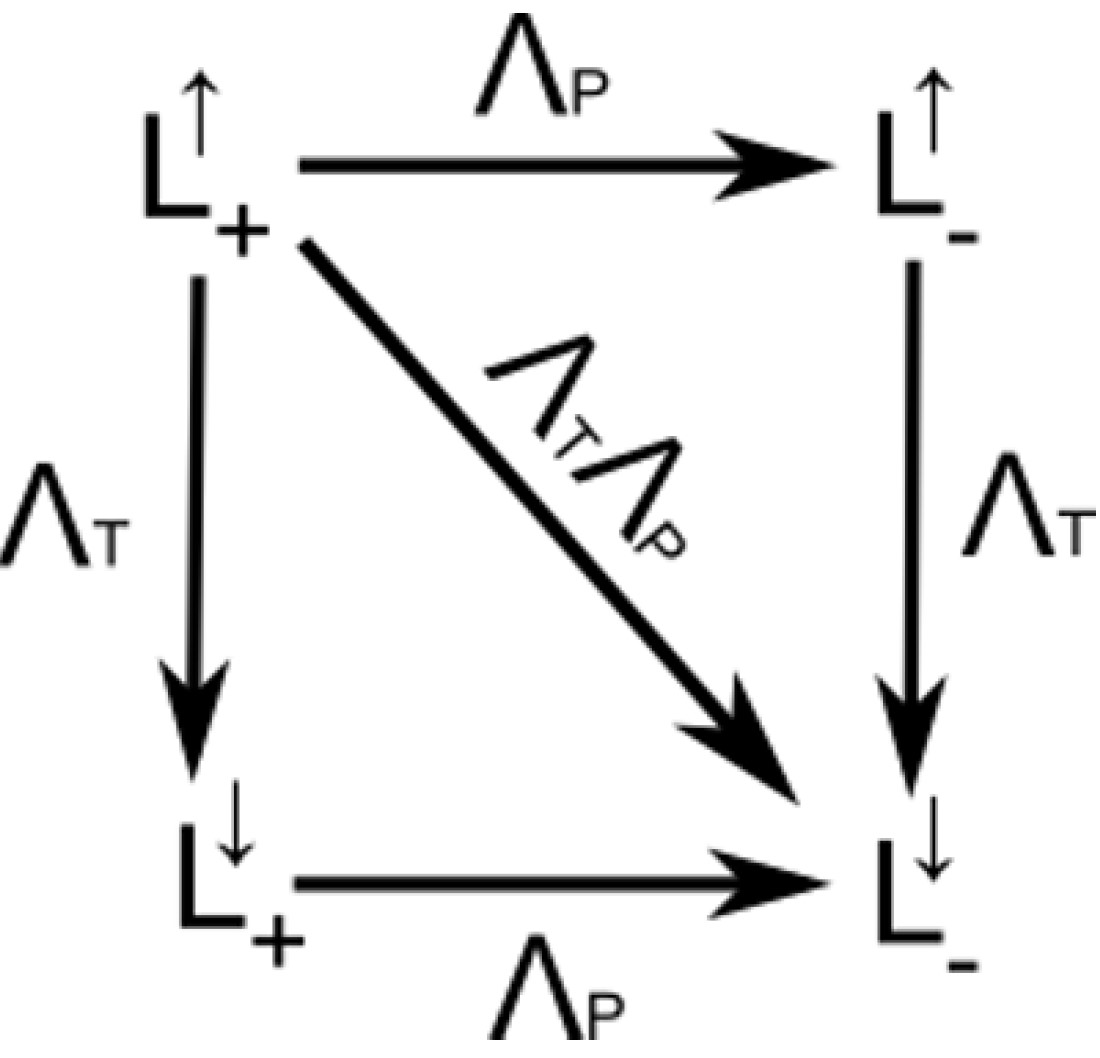
\includegraphics[width=0.3\columnwidth]{figures/lorentz-group-components.jpg}  
\end{center}
\caption{Components of the Lorentz group. Elements of the Lorentz group outside of the proper orthochronous Lorentz group are connected via the discrete ``jumps'' $\Lambda_P$ and $\Lambda_T$.}
\label{fig:lorentz-group-components}
\end{figure}

\subsection{Representation of the Lorentz group}
A representation of the Lorentz group can be broken down into 6 generators: 3 generators for \textbf{rotations} and 3 generators for \textbf{boosts}.

Rotations in space leave the time of an event unchanged. Such transformations obey the characteristic equation of Lorentz transforms Eq.\eqref{eq:lorentz-tfm-characteristic}. We can write down the 3 generators of the rotations $J_i$ as
\begin{equation}
J_i =  \begin{pmatrix}
0&\\
&J_i^{3dim}
\end{pmatrix} \label{eq:representation-rotation-lorentz}
\end{equation}
where $J_i^{3dim}$ obey the commutation relations in Eq.\eqref{eq:lie-bracket-so3}. It follows that $J_i$ also obey these commutation relations.

For the 3 generators of boosts, $K_i$, consider a series expansion of $\tensor{\Lambda}{^\mu_\rho}$, and take the first linear term for an infinitesimal Lorentz transformation 
\begin{equation}
\tensor{\Lambda}{^\mu_\rho} \approx \tensor{\delta}{^\mu _\rho} + \epsilon \tensor{K}{^\mu _\rho} + ...
\end{equation}
Substituting this into Eq.\eqref{eq:lorentz-tfm-characteristic}, we end up with
\begin{align}
\eta_{\sigma \nu} \tensor{K}{^\sigma _\mu} + \eta_{\mu \delta} \tensor{K}{^\delta _\nu}   &= 0 \\
\tensor{K}{^\sigma _\mu} \eta_{\sigma \nu} + \eta_{\mu \delta} \tensor{K}{^\delta _\nu}   &= 0
\end{align}
Noting that $\tensor{C}{^i_j} = \tensor{A}{^i_k}\tensor{A}{^k_j}$ and using the definition of the transpose (see e.g. Eq.\eqref{eq:complicated-example-matrix-mul-transp}),
\begin{align}
\tensor{(\protect{K^T})}{^\mu _\sigma} \tensor{\eta}{_\sigma _\nu} + \tensor{\eta}{_\mu_\delta} \tensor{K}{^\delta _\nu}   &= 0 \\
(\boldsymbol{K}^T\boldsymbol{\eta})_{\mu \nu} + (\boldsymbol{\eta K})_{\mu \nu}   &= 0 \\
\boldsymbol{K}^T\boldsymbol{\eta} = - \boldsymbol{\eta K}. \label{eq:condition-generators-lt}
\end{align}

The transformations generated by $K$ are called \textbf{boosts}: namely a change into a coordinate system that moves with a different velocity with respect to the original coordinate system. Now we know, physically, that we can boost into frames which are moving relative to the original frame in some combination of the $x$, $y$, and $z$ axes. A boost in the $x$-direction only should leave the location of events in the $y$ and $z$ directions unchanged. From this information, we can derive a basis for the generators $K$ from Eq.\eqref{eq:condition-generators-lt}
\begin{equation}
K_1 = \begin{pmatrix}
0 & i & 0 & 0 \\
i & 0 & 0 & 0 \\
0 & 0 & 0 & 0 \\
0 & 0 & 0 & 0 \\
\end{pmatrix}\ 
K_2 = \begin{pmatrix}
0 & 0 & i & 0 \\
0 & 0 & 0 & 0 \\
i & 0 & 0 & 0 \\
0 & 0 & 0 & 0 \\
\end{pmatrix}\
K_3 = \begin{pmatrix}
0 & 0 & 0 & i \\
0 & 0 & 0 & 0 \\
0 & 0 & 0 & 0 \\
i & 0 & 0 & 0 \\
\end{pmatrix}. \label{eq:representation-boost-lorentz}
\end{equation}
Exponentiation of these generators through $\Lambda = e^{i \phi K}$ yield
\begin{align}
\Lambda_1 = \begin{pmatrix}
\cosh(\phi) & -\sinh(\phi) & 0 & 0 \\
-\sinh(\phi) & \cosh(\phi) & 0 & 0 \\
0 & 0 & 1 & 0 \\
0 & 0 & 0 & 1 \\
\end{pmatrix}\ 
\Lambda_2 = \begin{pmatrix}
\cosh(\phi) & 0 &  -\sinh(\phi) & 0 \\
0 & 1 & 0 & 0 \\
 -\sinh(\phi) & 0 & \cosh(\phi) & 0 \\
0 & 0 & 0 & 1 \\
\end{pmatrix}\nonumber \\
\Lambda_3 = \begin{pmatrix}
\cosh(\phi) & 0 & 0 & -\sinh(\phi) \\
0 & 1 & 0 & 0 \\
0 & 0 & 1 & 0 \\
-\sinh(\phi) & 0 & 0 & \cosh(\phi) \\
\end{pmatrix}.
\end{align}

We can derive the other components of the Lorentz group by operating the parity and time reversal operators Eq.\eqref{eq:parity-time-reversal-operators} on each index of the generators. We find
\begin{align}
K_i \underbrace{\rightarrow}_P - K_i \label{eq:tfm-boost-parity} \\
K_i \underbrace{\rightarrow}_T - K_i.
\end{align}
A similar exercise can be done for transformations involving only rotations in space, and we find that the generators $J$ of these transformations are invariant under parity and time reversal.

\subsection{Lie algebra of the proper orthochronous Lorentz group}
From the explicit forms Eq.\eqref{eq:representation-rotation-lorentz} and Eq.\eqref{eq:representation-rotation-lorentz} we can derive the Lie algebra of $L_+^\uparrow$ by brute force, to give
\begin{align}
[J_i, J_j] &= i \epsilon_{ijk} J_k \label{eq:commutator-rotation-rotation}\\
[J_i, K_j] &= i \epsilon_{ijk} K_k \label{eq:commutator-rotation-boost}\\
[K_i, K_j] &= -i \epsilon_{ijk} J_k.\label{eq:commutator-boost-boost}
\end{align}
Eq.\eqref{eq:commutator-rotation-rotation} shows us that rotation generators are closed under commutation, whereas none of the other combinations are. Note also that a general proper orthochronous Lorentz transformation is of the form
\begin{equation}
\Lambda = e^{i \boldsymbol{J}\cdot \boldsymbol{\theta} + i \boldsymbol{K}\cdot \boldsymbol{\phi}}.
\end{equation}

We now complexify the Lie algebra, changing the basis into components of the Lie algebra's two ``ideals'' $N^+$ and $N^-$:
\begin{equation}
N_i^\pm = \frac{J_i \pm i K_i}{2}. \label{eq:complexification-lie-algebra-lorentz-group}
\end{equation}
These generators are now separately closed under commutation, and also commute with each other
\begin{align}
[N_i^+, N_j^+] &= i \epsilon_{ijk} N_k^+ \\
[N_i^-, N_j^-] &= i \epsilon_{ijk} N_k^- \\
[N_i^+, N_j^-] &= 0. 
\end{align}
Notice that the first two commutation relations are precisely the commutation relations we derived for $SU(2)$ in Eq.\eqref{eq:lie-bracket-su2}! We have therefore discovered that the complexified Lie algebra of $L^\uparrow_+$ consists of two copies of the Lie algebra of the complexification of $\mathfrak{su}(2)$. Technically, we have shown that
\begin{equation}
\mathfrak{so}(1,3)_\mathbb{C}  \cong \mathfrak{sl}(2, \mathbb{C}) \oplus \mathfrak{sl}(2, \mathbb{C})
\end{equation}
where $\mathfrak{sl}(2, \mathbb{C})$ is the complexification of $\mathfrak{su}(2)$, $\cong$ denotes an isomorphism, and $\oplus$ denotes the direct sum of a Lie algebra (see Defn.~\ref{defn:direct-sum-lie-algebra}).

\begin{defn}[Direct sum of two Lie algebras] \label{defn:direct-sum-lie-algebra}
For two Lie algebras $\mathfrak{g}$ and $\mathfrak{g}'$, their direct sum Lie algebra is the vector space $\mathfrak{g} \oplus \mathfrak{g}'$ consisting of all pairs $(x, x')$, $x \in \mathfrak{g}$, $x' \in \mathfrak{g'}$, with the operation
\begin{equation}
[(x, x'), (y, y')] = ([x,y], [x',y'])
\end{equation}
such that copies of $\mathfrak{g}$ and $\mathfrak{g}'$ commute with each other
\begin{equation}
[(x,0),(0,x')] = 0. 
\end{equation}
\end{defn}

In Section~\ref{sec:finite-dim-irr-repr} we found that we can label each irreducible representation of $\mathfrak{su}(2)$ by the scalar value of the Casimir element (see Eq.\eqref{eq:connection-max-eval-cartan-and-casimir-element-su2}, we will simply use $j$ instead of $j(j+1)$). Since the Lorentz group consists of two copies of $\mathfrak{su}(2)$, we need two labels to label each irreducible representation of the Lorentz group: $j_1$ and $j_2$ where $j_1, j_2 = 0, 1/2, 1, 3/2, ...$.

Finally, note that it is conventional to write the Lie algebra of the Lorentz group more compactly as 
\begin{align}
J_i &= \frac{1}{2} \epsilon_{ijk} M_{jk} \label{eq:defn-compact-lorentz-lie-algebra-notation} \\
K_i &= M_{0i} 
\end{align}
where
\begin{equation}
[\tn{M}{_\mu_\nu},\tn{M}{_\rho_\sigma}] = i(\tn{\eta}{_\mu _\rho} \tn{M}{_\nu _\sigma} - \tn{\eta}{_\mu _\sigma} \tn{M}{_\nu _\rho} - \tn{\eta}{_\nu _\rho} \tn{M}{_\mu _\sigma} + \tn{\eta}{_\nu _\sigma} \tn{M}{_\mu _\rho}). \label{eq:lorentz-algebra}
\end{equation}

\subsection{Finite dimensional irreducible representations of the Lorentz group}
We denote the finite dimensional irreducible representations of the Lorentz group as $(j_1, j_2)$ where $j_1$ corresponds to the Casimir element of the $N^+$ copy of $SU(2)$, and $j_2$ corresponds to the Casimir element of the $N^-$ copy in Eq.\eqref{eq:complexification-lie-algebra-lorentz-group}.

\subsubsection{The $(0,0)$ representation}
This is the lowest dimensional representation. Both copies of $SU(2)$ are 1-dimensional, and the only 1$\times$1 matrices that fulfils the commutation relations is the number 0. Hence
\begin{equation}
N_i^+ = N_i^- = 0
\end{equation}
corresponding to the identity. The $(0,0)$ representation therefore acts on objects, called \textbf{Lorentz scalars}, that do not change under Lorentz transformations. This is called the \textbf{scalar representation}. Examples of Lorentz scalars turn out to be spacetime distance between two events; the length of 4-velocities; and the Ricci curvature in a point in spacetime (from General relativity). 

\subsubsection{The $(\frac{1}{2},0)$ representation}
In this representation, we use the 2-dimensional representation for one copy of $SU(2)$ $N_i^+ = \sigma_i/2$ (see Eq.\eqref{eq:generator-su2-lie-algebra-2d}), and the 1-dimensional representation for the other $N_i^-=0$. Using Eq.\eqref{eq:complexification-lie-algebra-lorentz-group} we find
\begin{align}
J_i &= \frac{\sigma_i}{2} \\
K_i &= \frac{-i}{2} \sigma_i.
\end{align}
Letting rotations be denoted by $R_i(\theta)$ and boosts by $B_i(\phi)$, we have
\begin{align}
R_i(\theta) &= e^{\frac{i \theta}{2}  \sigma_i} \\
B_i(\phi) &= e^{\frac{\phi}{2}  \sigma_i}.
\end{align}
So, for example, writing out explicitly the form of $R_1(\theta) \equiv R_x(\theta)$, we have
\begin{equation}
R_x(\theta) = \begin{pmatrix}
\cos(\theta/2) & i \sin(\theta/2) \\
i \sin(\theta/2) & \cos(\theta/2)
\end{pmatrix}. \label{eq:rotation-left-chiral-lorentz-tfm}
\end{equation}
Contrast this to the 2D rotation matrix in Eq.\eqref{eq:2d-rotation-matrix}: we see that \textbf{we must rotate this object by $4\pi$ to get an identity transform}! It is clear that the object which such transformations operate on \textbf{are not} simple two-dimensional vectors, or indeed even 4-vectors of Minkowski space. The \textbf{two-component} object  this representation acts upon are called \textbf{left-chiral spinors}.
\begin{defn}[Left-chiral spinor]
Is an object that transforms under the $(\frac{1}{2},0)$ representation of the Lorentz group. We denote them as 
\begin{equation}
\chi_L = \begin{pmatrix}
(\chi_L)_1 \\
(\chi_L)_2 
\end{pmatrix}.
\end{equation}
\end{defn}
\noindent We will see later that the two components of this object correspond to \textbf{spin-up} and \textbf{spin-down}. 

Notice how the factor of $\theta/2$ in Eq.\eqref{eq:rotation-left-chiral-lorentz-tfm} means that rotation of a spinor by $2\pi$ gives a minus sign. A spinor must be rotated by $4\pi$ to get the identity transform. We saw from the previous section that the lowest-dimensional representation of the Lorentz group is always the identity, and therefore trivial. Hence, we may say that \textbf{a spinor is the simplest object that can be Lorentz-transformed} \citep{Steane13}.

\subsubsection{The $(0, \frac{1}{2})$ representation}
This follows identically to the previous section, except with $N_i^+=0$ and $N_i^- = \sigma_i/2$. 
\begin{align}
J_i &= \frac{\sigma_i}{2} \\
K_i &= \frac{i}{2} \sigma_i.
\end{align}
So,
\begin{align}
R_i(\theta) &= e^{\frac{i \theta}{2}  \sigma_i} \\
B_i(\phi) &= e^{-\frac{\phi}{2}  \sigma_i}.
\end{align}
We see rotations under this representation are identical to the $(\frac{1}{2},0)$ representation, but boosts differ by a minus sign in the exponent. Hence, objects which transform under the $(0, \frac{1}{2})$ representation are \textbf{similar but not identical to} left-chiral spinors.
\begin{defn}[Right-chiral spinor]
Is an object that transforms under the $(0, \frac{1}{2})$ representation of the Lorentz group. We denote them as 
\begin{equation}
\chi_R = \begin{pmatrix}
(\chi_R)^1 \\
(\chi_R)^2 
\end{pmatrix}.
\end{equation}
\end{defn}
\noindent The generic name for left- and right-chiral spinors is \textbf{Weyl spinors}.

\subsubsection{Van der Waerden Notation}

Van der Waerden Notation introduces dotted indices to distinguish chirality.

\begin{defn}[Undotted indices (chiral indices)]
Define a left-chiral spinor with a lower, undotted, index
\begin{equation}
\chi_L = \chi_a
\end{equation}
\end{defn}

\begin{defn}[Dotted indices (anti-chiral indices)]
Define a right-chiral spinor with an upper, dotted, index
\begin{equation}
\chi_R = \chi^{\dot{a}}
\end{equation}
\end{defn}

\begin{defn}[Spinor metric]
The spinor metric is defined as 
\begin{equation}
\tn{\epsilon}{^a^b} = i \tn{(\sigma_y)}{^a^b} = \begin{pmatrix}
0 & 1 \\
-1 & 0
\end{pmatrix}
\end{equation}
and with lower indices
\begin{equation}
\tn{\epsilon}{_a_b} = (\tn{\epsilon}{^a^b})^T = \begin{pmatrix}
0 & -1 \\
1 & 0
\end{pmatrix}
\end{equation}
\end{defn}

Using the manner in which left and right chiral spinors Lorentz transform, we can show that
\begin{equation}
\chi^{\dot{a}} = \tn{\epsilon}{^a^b} \chi^*_a
\end{equation}
where $^*$ denotes complex conjugation. We therefore have the rule that complex conjugation transforms an undotted index into a dotted index, and vice versa:
\begin{align}
(\chi^{\dot{a}})^* &= \chi^a  \\
\chi_a^* &= \chi_{\dot{a}}.
\end{align}
We also find, using the fact that the Pauli matrices are Hermitian ($\sigma^\dagger = \sigma$), that the dot product of spinors of the same type are Lorentz invariant. E.g.
\begin{align}
{\chi'}_a^T {\chi'}^a = \chi_a^T \chi^a = \chi_a^T \tn{\epsilon}{^a^b}\chi_b \\
{\chi'}_{\dot{a}}^T {\chi'}^{\dot{a}} = \chi_{\dot{a}}^T \chi^{\dot{a}} = \chi_{\dot{a}}^T \tn{\epsilon}{^a^b}\chi_{\dot{b}}.
\end{align}

We can thus define the following notation for Lorentz transforming Weyl spinors:
\begin{align}
\Lambda_{(\frac{1}{2},0)} &=  e^{i \frac{\theta}{2}\sigma + \frac{\phi}{2} \sigma} = \tn{\Lambda}{_a^b}  \\
\Lambda_{(0, \frac{1}{2})} &=  e^{i \frac{\theta}{2}\sigma - \frac{\phi}{2} \sigma} = \tn{\Lambda}{^{\dot{a}}_{\dot{b}}}. \label{eq:weyl-spinor-lt}
\end{align}
\textbf{[TODO: I do not understand i) the significance (if any) of the left/right position of the indices in this notation; ii) If the spinor metric also raises/lowers indices of the Lorentz transform. Proceed with caution!]} So,
\begin{align}
\chi'_R = \chi'^{\dot{a}} = \tn{\Lambda}{^{\dot{a}}_{\dot{b}}} \chi^{\dot{b}} \\
\chi'_L = \chi'_{a} = \tn{\Lambda}{_a^b} \chi_b. \\
\end{align}

\subsubsection{The $(\frac{1}{2},\frac{1}{2})$ representation}
Let's denote the object which transforms under this representation as $\tn{v}{_a^{\dot{b}}}$ using Van der Waerden notation. Since the two copies of $SU(2)$ do not commute within the representation (we have a direct sum), they will not interfere with each other and so we can transform the indices separately. We know that, since we have two copies of $\mathfrak{su}(2)$ with $j=1/2$, that $\tn{v}{_a^{\dot{b}}}$ must have four elements, since each copy of $\mathfrak{su}(2)$ must have two associated states (corresponding to $m=\pm 1/2$, see Section~\ref{sec:finite-dim-irr-repr}).

We will assume\footnote{The justification for the assumption by Schwichtenberg was unclear and seemed circular to me, so I omit it.} that the irreducible representation acts on 2$\times$2 Hermitian matrices. This is because 2D Hermitian matrices only have 4 degrees of freedom, which coincides with the number of elements we argued that $\tn{v}{_a^{\dot{b}}}$ must have. Any 2D Hermitian matrix may be decomposed in terms of Pauli matrices which form a basis together with the identity:
\begin{equation}
a_0 1 + a_i \sigma_i.
\end{equation}


For convenience, we first work with $\tn{v}{_a_{\dot{b}}}$, and can use the spinor metric to raise the right index later. By decomposing $\tn{v}{_a_{\dot{b}}}$ in terms of Pauli matrices, we have
\begin{equation}
\tn{v}{_a_{\dot{b}}} = \begin{pmatrix}
v_0 + v_3 & v_1 - i v_2 \\
v_1 + i v_2 & v_0 - v_3
\end{pmatrix}.
\end{equation}
We now observe how this object Lorentz transforms
\begin{equation}
\tn{{v'}}{_a_{\dot{b}}} = \tn{\Lambda}{_a^c} \tn{{v}}{_c_{\dot{d}}} \tn{\Lambda}{^{\dot{d}}_{\dot{b}}}
\end{equation}
corresponding to (using Eq.\eqref{eq:weyl-spinor-lt})
\begin{equation}
v \rightarrow v' = \tn{{v'}}{_a_{\dot{b}}} = \tn{{\left(e^{i \vec{\theta} \frac{\vec{\sigma}}{2} + \vec{\phi} \frac{\vec{\sigma}}{2}} \right)}}{_a^c} \tn{v}{_c_{\dot{d}}} \tn{{\left(e^{i \vec{\theta} \frac{\vec{\sigma}}{2} - \vec{\phi} \frac{\vec{\sigma}}{2}} \right)}}{^{\dot{d}}_{\dot{b}}} 
\end{equation}
[\textbf{TODO: Apparently this is Hermitian but I'm having difficulty proving it... The $i$ in the exponent makes it look very not Hermitian to me...}] It turns out, after doing this transformation, that you get exactly the same components as a boosted 4-vector. Therefore the $(\frac{1}{2},\frac{1}{2})$ representation of $SU(2)$ is exactly the same thing as $SO(1,3)$. Furthermore, \textbf{we see that 4-vectors are not fundamental}, and thus there are physical systems which cannot be described by 4-vectors. In this sense, people sometimes call spinors the square root of 4-vectors: in the same way that vectors are square roots of rank-2 tensors.

\subsubsection{Dirac and Majorana spinors}
We know from Eq.\eqref{eq:tfm-boost-parity} that boosts obtain a sign change under parity transformations. Furthermore, by definition of the generators of the Lorentz group Eq.\eqref{eq:complexification-lie-algebra-lorentz-group} that parity transformations therefore flip $N^+ \leftrightarrow N^-$. This is the motivation for calling the two kinds of Weyl spinor left- and right-handed.

\begin{defn}[Dirac spinor]
A Dirac spinor is a concatenation of a left-chiral Weyl spinor with an \textbf{independent} right-chiral Weyl spinor
\begin{equation}
\Psi = \begin{pmatrix}
\chi_L \\
\xi_R
\end{pmatrix} = 
\begin{pmatrix}
\chi_a \\
\xi^{\dot{a}}
\end{pmatrix}
\end{equation}
where the independence of the two components is denoted by the different symbols $\chi$ and $\xi$.
\end{defn}

Dirac spinors transform simply by constructing a block-diagonal matrix of transformations for the $(\frac{1}{2},0)$ and $(0, \frac{1}{2})$ representations, since the two constituent Weyl spinors transform independently:
\begin{equation}
\Psi \rightarrow \Psi' = \Lambda_{(\frac{1}{2},0) \oplus (0, \frac{1}{2})} \Psi = \begin{pmatrix}
\Lambda_{(\frac{1}{2},0)} & 0 \\
0 & \Lambda_{(0, \frac{1}{2})} 
\end{pmatrix} \begin{pmatrix}
\chi_L \\
\xi_R
\end{pmatrix}.
\end{equation}

\begin{defn}[Majorana spinor]
A Majorana spinor is a special case of a Dirac spinor
\begin{equation}
\Psi = \begin{pmatrix}
\chi_L \\
\chi_R
\end{pmatrix} = 
\begin{pmatrix}
\chi_a \\
\chi^{\dot{a}}
\end{pmatrix}.
\end{equation}
\end{defn}

If a transformation which operates on a Dirac spinor is invariant to parity, then we will be able to say that that transformation is invariant to parity. Hence, it is useful to observe how Dirac spinors transform under parity. Since parity transforms result in $N^+ \leftrightarrow N^-$, then
\begin{equation}
\left(\frac{1}{2}, 0\right) \underbrace{\leftrightarrow}_{P} \left(0, \frac{1}{2}\right).
\end{equation}
So, instead of transforming under the $(\frac{1}{2},0) \oplus (0, \frac{1}{2})$ representation, a parity transformed Dirac spinor transforms under the $(0, \frac{1}{2}) \oplus (\frac{1}{2},0)$ representation
\begin{equation}
\Psi^P \rightarrow (\Psi^P)' = \Lambda_{(0, \frac{1}{2}) \oplus (\frac{1}{2},0)} \Psi^P = \begin{pmatrix}
\Lambda_{(0, \frac{1}{2})} & 0 \\
0 & \Lambda_{(\frac{1}{2},0)} 
\end{pmatrix} \begin{pmatrix}
\xi_R \\
\chi_L
\end{pmatrix}.
\end{equation}
Hence, a parity transformation has the following effect on a Dirac spinor
\begin{equation}
\Psi = \begin{pmatrix}
\chi_L \\
\xi_R
\end{pmatrix} \underbrace{\rightarrow}_P
\Psi^P = \begin{pmatrix}
\xi_R \\
\chi_L
\end{pmatrix}.
\end{equation}
Note that this is \textbf{not} the same as $\chi_L \rightarrow \chi_R$, which we discuss next. 

\subsubsection{Spinor charge conjugation}
\begin{defn}
Given a Dirac spinor $\Psi$
\begin{equation}
\Psi = \begin{pmatrix}
\chi_L \\
\xi_R
\end{pmatrix}
\end{equation}
we define the charge conjugate spinor as 
\begin{equation}
\Psi^C = \begin{pmatrix}
\xi_L \\
\chi_R
\end{pmatrix}.
\end{equation}
\end{defn}

Note that a charge conjugate spinor still Lorentz transforms like a Dirac spinor, according to $\Lambda_{(\frac{1}{2},0) \oplus (0, \frac{1}{2})}$. We show later that charge conjugation flips \textbf{all} labels used to describe fundamental particles (not just electric charge). We can see, for example, that a left-chiral spinor would be transformed into a right-chiral spinor under charge conjugation. 

\subsection{Infinite-dimensional representations of the Lorentz group}
So far we've considered transformations on objects $\Phi_a$ of the form
\begin{equation}
\Phi_a \rightarrow \Phi_a' = M_{ab}(\Lambda)\Phi_b
\end{equation}
where $M_{ab}$ denotes a particular finite-dimensional representation of the Lorentz transformation $\Lambda$. However, objects in physics dynamically change with space and time. Therefore, our objects must become functions of coordinates $\Phi = \Phi(x)$, where the coordinates themselves are also affected by Lorentz transformations. Hence\footnote{Though most authors use the Wigner convention for symmetry operators: $\Phi_a'(x) = M_{ab}(\Lambda)\Phi_b(\Lambda^{-1} x)$}
\begin{equation}
\Phi_a(x) \rightarrow \Phi_a'(x) = M_{ab}(\Lambda)\Phi_b(\Lambda x).
\end{equation}
Our transformations therefore consist of two parts. One part, represented by a finite-dimensional representation, acting on $\Phi_a$; a second part that transforms the spacetime coordinates. We therefore need an infinite number of basis functions to decompose the object $\Phi_a(x)$ -- which is the idea behind Fourier transforms. 

\begin{defn}[Infinite-dimensional representation of the Lorentz group]
The generator of the infinite-dimensional representation of the Lorentz group is given by differential operators
\begin{equation}
\tn{{M^{\text{inf}}}}{_\mu_\nu} = i(x^\mu \partial^\nu - x^\nu \partial^\mu)
\end{equation}
\end{defn}
Note that we can plug $\tn{{M^{\text{inf}}}}{_\mu_\nu}$ into Eq.\eqref{eq:lorentz-algebra} to show that it does indeed satisfy the definition of the Lorentz algebra.

The complete transformation is then a combination of a finite-dimensional representation $\tn{{M^{\text{fin}}}}{_\mu_\nu}$ and an infinite-dimensional transformation
\begin{equation}
\Phi_a(x) \rightarrow \tn{{\left( e^{-\frac{i}{2} \omega^{\mu \nu} \tn{{M^{\text{fin}}}}{_\mu_\nu}} \right)}}{_a^b}  e^{-\frac{i}{2} \omega^{\mu \nu} \tn{{M^{\text{inf}}}}{_\mu_\nu}} \Phi_b(x)
\end{equation}
where the extent of rotation $\theta_i$ and boost $\phi_i$ correspond to
\begin{align}
\theta_i &= \frac{1}{2}\tn{\epsilon}{_i_j_k} \tn{\omega}{_j_k} \\
\phi_i &= \tn{\omega}{_0_i}
\end{align}
(see Eq.\eqref{eq:defn-compact-lorentz-lie-algebra-notation}). Since the matrices $ \tn{{M^{\text{fin}}}}{_\mu_\nu}$ are finite dimensional and constant, we can [apparently] put the two components together:
\begin{defn}[Field representation of the Lorentz group]
The field representation of the Lorentz group is given by:
\begin{align}
\Phi_a(x) &\rightarrow \tn{{\left( e^{-\frac{i}{2} \omega^{\mu \nu} \tn{M}{_\mu_\nu}} \right)}}{_a^b}   \Phi_b(x) \\
\tn{M}{_\mu_\nu} &= \tn{{M^{\text{fin}}}}{_\mu_\nu} + \tn{{M^{\text{inf}}}}{_\mu_\nu}.
\end{align}
\end{defn}

\subsection{The Poincar\'{e} group}

We are now in a position to discuss \textbf{translations}. Translations to not mix components, so we do not need a finite-dimensional representation of the group of translations. The Lorentz group plus\footnote{Technically, the Poincar\'{e} group is the semi-direct sum of the Lorentz group and translations.} the group of translations is called the \textbf{Poincar\'{e} group}. A one-dimensional infinitesimal translation of a function along the $x$-axis is given by
\begin{equation}
\Phi(x) \rightarrow \Phi(x+\epsilon) = \Phi(x) + \partial_x \Phi(x) \epsilon
\end{equation}
(which is the Taylor expansion of $\Phi(x+\epsilon)$ to first order). In physics, it is convenient to define an $i$ with the generator
\begin{align}
P_i &\equiv -i \partial_i \\
P_0 &\equiv i \partial_0 \\
\implies P_\mu &= i \eta^{\mu \nu} \partial_\nu.
\end{align}
Hence an arbitrary finite translation of an object by $a^i$ is given by
\begin{equation}
\Phi(x) \rightarrow \Phi(x+a) = e^{-ia^iP_i}\Phi(x) = e^{-a^i\partial_i}\Phi(x).
\end{equation}
Writing this as a Taylor expansion simply yields the Taylor expansion of $\Phi(x+a)$. To translate to another point in time we use $P_0$.

The Lie algebra of the Poincar\'{e} group is
\begin{align}
[J_i, J_j] = i \epsilon_{ijk}J_k \\
[J_i, K_j] = i \epsilon_{ijk} K_k \\
[K_i, K_j] = -i \epsilon_{ijk} J_k \\
[J_i, P_j] = i \epsilon_{ijk} P_k \\
[J_i, P_0] = 0 \\
[K_i, P_j] = i \delta_{ij} P_0 \\
[K_i, P_0] = -i P_i.
\end{align}
More succinctly, along with Eq.\eqref{eq:lorentz-algebra} we have the additional commutation relations
\begin{align}
[P_\mu, P_\nu] &= 0 \\
[\tn{M}{_\mu_\nu}, P_\rho] &= i (\tn{\eta}{_\mu_\rho} P_\nu - \tn{\eta}{_\nu_\rho}P_\mu)
\end{align}

It turns out that the Poincar\'{e} group has two Casimir operators. The first one is
\begin{equation}
P_\mu P^\mu \defeq m^2.
\end{equation}
We will find out later that $m$ coincides with the \textbf{mass} of particles. The second Casimir operator is
\begin{align}
W_\mu & W^\mu  \\
W^\mu &= \frac{1}{2} \epsilon^{\mu \nu \rho \sigma} P_\nu M_{\rho \sigma}
\end{align}
where $W^\mu$ is called a \textbf{Pauli-Lubanski four-vector}. It can be shown that $j \equiv j_1 + j_2$ can be used as a label (where each $j_i$ corresponds to a representation of $SU(2)$), which we refer to as the \textbf{spin} $j$ representation. $W^\mu$ describes spin states of moving particles. So, overall, each representation is labelled by two scalar values: $m$ and $j$. $m$ can take arbitrary values whereas $j$ is restricted to half-integers.

\subsection{Elementary particles}
The labels for the irreducible representations of the double cover of the Poincar\'{e} group, mass $m$ and spin $j$, are how elementary particles are labelled in physics. More labels, called charges, will follow later from internal symmetries\footnote{An internal symmetry is a transformation acting only on the fields, therefore not transforming spacetime points, and leaving the lagrangian or the physical results invariant.}: electric charge, weak isospin, and color charge. 

The particles of the standard model are one of:
\begin{itemize}
\item Spin 0, described by an object $\Phi$, called a \textbf{scalar}, that transforms according to the $(0,0)$ representation of the Lorentz group, called the \textbf{spin $0$ representation}, or scalar representation. The Higgs particle is described by a scalar field.
\item Spin $\frac{1}{2}$, described by an object $\Psi$, called a \textbf{spinor}, transforms according to the $(\frac{1}{2}, 0) \oplus (0, \frac{1}{2})$ representation, called the \textbf{spin $\frac{1}{2}$ representation}, or spinor representation. Electrons and quarks are described by spinors.
\item Spin 1, is described by an object $A$, called a \textbf{vector}, that transforms according to the $(\frac{1}{2}, \frac{1}{2})$ representation, called the \textbf{spin 1 representation}, or vector representation. Photons are described by vectors.
\end{itemize}

\section{The framework: field theory}
The underlying idea of field theory is that Nature minimizes \textit{something}. This something must be Lorentz invariant (otherwise we would get different equations of motion for fields for different observers). It will turn out that this \textit{something} is the simplest possible choice of Lorentz invariant.

\subsection{The least action principle}
\begin{defn}[Action (classical mechanics)]
The action of a physical system $S$ under classical mechanics is defined as
\begin{equation}
S[q(t)] = \int_{t_1}^{t_2} \mathcal{L}(q(t), \dot{q}(t), t) \d{t}
\end{equation}
where $q(t)$ is a position vector with some finite number of degrees of freedom, and $\mathcal{L}$ is called the \textbf{Lagrangian}.
\end{defn}

Note that, in some theories we will go on to consider, we cannot derive a Lorentz-invariant theory by only considering up to the first-order derivative of $q(t)$ and will have to go to second order. \textbf{Ostrogradsky instability} prevents us from considering theories with more than two time derivatives, since they correspond to Hamiltonians unbounded from below. It is also interesting to note that a theory with an infinite number of derivatives would allow a non-local theory\footnote{A non-local theory is one which admits interactions of the form $\Phi(x)\Phi(x-h)$ for some arbitrary distance $h$}. Furthermore, in order to get a free (non-interacting) theory of particles/fields, the Lagrangian must stop at the lowest-order non-trivial derivative.

\begin{defn}[Least action principle]
The principle of least action states that the equations of motion correspond to
\begin{equation}
\delta S = 0
\end{equation}
where $\delta$ means a \textit{small} change: meaning that the action is stationary to first order for sufficiently short, finite segments in the path.
\end{defn}

\begin{defn}[Lagrangian density]
Define the Lagrangian density $\mathscr{L}$ as
\begin{equation}
\mathcal{L} = \int \mathscr{L} \dpow{x}{3}
\end{equation}
\end{defn}

In \textbf{field theories}, we do not use the position/momentum of particles to derive equations of motion, but instead fields $\Phi(\vec{x},t)$, where the action becomes
\begin{defn}[Action (field theory)]
The action of a physical system $S$ under a field theory is defined as
\begin{equation}
S[\Phi(\vec{x}, t)] = \int \mathscr{L}(\Phi(\vec{x}, t), \partial_{\mu}\Phi(\vec{x}, t), \vec{x}, t) \dpow{x}{4}. \label{eq:action-field-theory}
\end{equation}
where $\Phi(\vec{x}, t)$ is a field.
\end{defn}
\noindent Notice that Eq.\eqref{eq:action-field-theory} treats space and time on an equal footing, since fields vary over both space and time. In contrast, for classical mechanics, we parametrized the dynamics of our particle with time only: $q(t)$ and $\dot{q}(t)$. 

\subsection{Euler-Lagrange equation}
Consider a classical path of a particle between fixed two points in time $t_1$ and $t_2$ that obeys the least action principal. We consider perturbing that path, and requiring that the difference in the action to first order vanishes. This yields the Euler-Lagrange equations.

Mathematically, first expand the perturbed Lagrangian around the point $(q, \dot{q}, t)$ using a double Taylor expansion
\begin{equation}
\mathcal{L}(q + \epsilon, \dot{q} + \dot{\epsilon}(t), t) = \mathcal{L}(q, \dot{q}, t) + (q + \epsilon - q)\pderiv{\mathcal{L}}{t} + (\dot{q} + \dot{\epsilon} - \dot{q})\pderiv{\mathcal{L}}{\dot{q}} + ...
\end{equation}
where $q = q(t)$, $\dot{q} = \dot{q}(t)$, $\epsilon = \epsilon(t)$. By demanding $\delta S = 0$, we have
\begin{equation}
\delta S = \left[ \int_{t_1}^{t_2} \mathcal{L}(q, \dot{q}, t) \d{t} \right]- \left[ \int_{t_1}^{t_2} \mathcal{L}(q + \epsilon, \dot{q} + \dot{\epsilon}, t) \d{t} \right] = 0
\end{equation}
So, substituting the first-order Taylor expansion, we have
\begin{equation}
\int_{t_1}^{t_2}\left( \epsilon \pderiv{\mathcal{L}}{q} + \dot{\epsilon} \pderiv{\mathcal{L}}{\dot{q}} \right) \d{t} = 0.
\end{equation}
We wish to factorize out $\epsilon(t)$ because it is an arbitrary perturbation. Using integration by parts on the term involving $\dot{\epsilon}$
\begin{equation}
\int \dot{\epsilon} \pderiv{\mathcal{L}}{\dot{q}} \d{t} = \cancel{\left.\pderiv{\mathcal{L}}{\dot{q}}\epsilon\right|_{t_1}^{t_2}} - \int \deriv{}{t}\left( \pderiv{\mathcal{L}}{\dot{q}} \right) \epsilon \d{t}
\end{equation}
where the first term cancels due to the assumption of fixed boundary conditions, so $\epsilon(t_1) = \epsilon(t_2) = 0$. We thus arrive at
\begin{equation}
\int_{t_1}^{t_2} \epsilon(t) \left[ \pderiv{\mathcal{L}}{q} - \deriv{}{t}\left( \pderiv{\mathcal{L}}{\dot{q}} \right) \right] \d{t} = 0
\end{equation}
and therefore we arrive at the famous Euler-Lagrange equation
\begin{equation}
\pderiv{\mathcal{L}(q, \dot{q}, t)}{q} - \deriv{}{t}\left( \pderiv{\mathcal{L}(q, \dot{q}, t)}{\dot{q}} \right) = 0. \label{eq:euler-lagrange-classical-mech}
\end{equation}
For (classical) field theory, we follow similar steps to obtain 
\begin{equation}
\pderiv{\mathscr{L}}{\Phi} - \partial_\mu \left( \pderiv{\mathscr{L}}{(\partial_\mu \Phi)} \right) = 0.
\end{equation}

\subsection{Noether's theorem}
Noether's theorem shows that each symmetry of the Lagrangian corresponds to a conserved quantity. This is one of the most beautiful insights in the history of science.

In order for dynamics to be invariant, the action must be invariant under a transformation of the Lagrangian. Consider some function $G(q)$ \textbf{[TODO: Or is it $G(q, \dot{q})$? Or $G(q, \dot{q}, t)$? Assuming he means what he says, $G(q)$]}. It turns out we can always add the total time derivative of a function to the Lagrangian
\begin{equation}
\mathcal{L} \rightarrow \mathcal{L} + \deriv{G}{t}
\end{equation}
because
\begin{equation}
\delta S \rightarrow \delta S + \int_{t_1}^{t_2} \d{t} \deriv{}{t} \delta G = \delta S + \cancel{\left. \pderiv{G}{q} \delta q \right|_{t_1}^{t_2}}
\end{equation}
due to the vanishing variation $\delta q$ at the boundaries.

Expanding $\delta \mathcal{L}$, and using the Euler-Lagrange equation Eq.\eqref{eq:euler-lagrange-classical-mech}, and rewriting with the product rule, yields
\begin{align}
J &= \pderiv{\mathcal{L}}{\dot{q}} \delta q + G \\
\deriv{}{t} J &= 0
\end{align}
And hence $J = \text{const}$, meaning that $J$ is \textbf{conserved with time}.

For example, for the Lagrangian $\mathcal{L} = m \dot{q}^2/2$, the Lagrangian is invariant under spatial translation $q \rightarrow q + a$. The corresponding conserved quantity is 
\begin{equation*}
J_\text{trans} = \pderiv{\mathcal{L}}{\dot{q}} a = m \dot{q} a.
\end{equation*}
$\deriv{}{t}J = 0$ holds for arbitrary $a$, and therefore momentum is conserved because the Lagrangian is invariant under spatial translations.

\newpage
\bibliography{physics-from-symmetry.bib} 

\end{document}
